% arara: clean: {extensions: ['log','idx','ilg','ind','out','bbl','blg','thm','toc','aux','pdf','synctex.gz','bcf','run.xml']}
% arara: lualatex: { shell: yes }
% arara: biber
% arara: lualatex: { synctex: yes }
% arara: makeindex
% arara: lualatex: { synctex: yes }
% arara: lualatex: { synctex: yes }
% arara: clean: {extensions: ['log','idx','ilg','ind','out','bbl','blg','thm','toc','aux','bcf','run.xml']}
\documentclass[graybox,envcountchap,sectrefs]{svmono}
% choose options for [] as required from the list
% in the Reference Guide

%\usepackage{mathptmx}
%\usepackage{helvet}
%\usepackage{courier}
%
\usepackage{type1cm}
\usepackage{makeidx}% allows index generation
\usepackage{graphicx}        % standard LaTeX graphics tool
															% when including figure files
\usepackage{multicol}        % used for the two-column index
\usepackage[bottom]{footmisc}% places footnotes at page bottom

\usepackage[lite]{mtpro2}
\usepackage{newtxtext}       % 
\usepackage{newtxmath}       % selects Times Roman as basic font
\usepackage{bm,dsfont}
\usepackage{mathrsfs}
\usepackage{lipsum}

\graphicspath{ {img} }

\usepackage[citestyle=numeric,style=numeric,backend=biber]{biblatex}
\addbibresource{bib.bib}

\usepackage{etoolbox,ifluatex}
\ifluatex
\makeatletter
\patchcmd{\PEX@}{\dp\Pbox@>\dp\z@}{\ht\Pbox@>\dp\z@}{}{}
\patchcmd{\SQEX@}{\dp\Sbox@>\dp0}{\ht\Sbox@>\dp0}{}{}
\makeatother
\fi

\DeclareMathOperator{\sen}{sen}
\newcommand{\divides}{\mid}
\newcommand{\notdivides}{\nmid}

\date{3 de mayo del 2019}
% see the list of further useful packages
% in the Reference Guide

\makeindex             % used for the subject index
                       % please use the style svind.ist with
                       % your makeindex program
%\let\claim\relax
%\renewcommand\claimname{Aa}
%%%%%%%%%%%%%%%%%%%%%%%%%%%%%%%%%%%%%%%%%%%%%%%%%%%%%%%%%%%%%%%%%%%%%
\begin{document}

\author{Carlos A. Aznarán Laos\\
Franss Cruz Ordoñez\\
Junior Micha Velasque\\
Gabriel Quiróz Gómez\\
Davis S. García Fernández}
\title{Relación de recurrencia}
\subtitle{-- Monografía de Análisis Real --}
\maketitle

\frontmatter%%%%%%%%%%%%%%%%%%%%%%%%%%%%%%%%%%%%%%%%%%%%%%%%%%%%%%
%\extrachap{A}
%\Extrachap{B}
\begin{dedication}
La presente monografía está dedicada a mis profesores y estudiantes de la Facultad de Ciencias.
\end{dedication}
\foreword
El problema \textsc{isoperimétrico}, un problema clásico visto en la antigüedad, lo que no necesita mucho de conocimiento matemático, en el que la proposición consiste: Dado
un número real positivo $L$, se trata de estudiar la cuestión siguiente: de todas las curvas cerradas del plano de longitud dada $L>0$, ¿cuál es la que encierra mayor área?
Esta cuestión puede ser respondida inclusive por personas que cursan el menor grado, en el que su intuición les indica que es la \emph{circunferencia}, la curva que encierra el mayor área y se sabe que la respuesta es $\tfrac{L^2}{4\pi}$. Pues ahí todo bien, la respuesta no era nada complicada. Pero el problema consiste en cómo se demostraría con matemáticas que la circunferencia maximiza el área, pues si se puede formar infinitas curvas con perímetro $L$. La materia de estudio del \textsc{cálculo variacional} consiste en buscar máximos y mínimos (o más generalmente extremos relativos) de funcionales continuos definidos sobre algún espacio funcional. También constituyen una generalización del cálculo elemental de máximos y mínimos de funciones reales de una variable.\par
\vspace{\baselineskip}
\begin{flushright}\noindent
Rímac, abril 2019\hfill {\it El profesor del curso}\\
\end{flushright}
\preface
Uno de los temas más importantes dentro del \emph{Análisis Matemático} son las sucesiones, es decir, funciones cuyo dominio y contradominio es el conjunto de los números naturales $\mathds{N}$ y el de los números reales $\mathds{R}$, respectivamente. En el presente trabajo nos enfocaremos en nada menos que las ``relaciones de recurrencia'', donde cualquier  término se determina en función de al menos uno de los términos precedentes, un ejemplo famoso es la \emph{sucesión de Fibonacci}. Esta sucesión fue descrita por \emph{Leonardo de Pisa}\footnote{Fibonacci} como la solución a un problema de cría de conejos:
\begin{quote}
	``Cierta persona cría una pareja de conejos juntos en un lugar cerrado y desea saber cuántos nacimientos durante un año han acontecido a partir del par inicial, de acuerdo a su naturaleza, cada pareja necesita un mes para envejecer y cada mes posterior procrea otra pareja''.
\end{quote}
Viendo esto, hemos concebido un modelo matemático basado en sucesiones recursivas, dando su definición, algunos otros ejemplos, su relación con las ecuaciones en diferencias y otras aplicaciones como resolver sistemas de ecuaciones lineales empleando nuestros conocimientos adquiridos en el curso de Análisis Real de la carrera de Matemática en la Universidad
Nacional de Ingeniería.
\vspace{\baselineskip}
\begin{flushright}\noindent
Rímac,\hfill {\it Carlos Aznarán Laos}\\
junio 2019\hfill {\it Franss Cruz Ordoñez}\\
\end{flushright}
\extrachap{Agradecimientos}
Nos gustaría expresar el agradecimiento especial al maestro Manuel Toribio Cangana, así como a nuestro profesor Benito Ostos, que nos brindó la excelente oportunidad de hacer este maravilloso proyecto sobre el tema de cálculo de variaciones, quien también me ayudó a hacer mucha investigación y llegué a conocer a muchos cosas nuevas. Estoy muy agradecido con ellos. En segundo lugar, también me gustaría agradecer a mis padres y amigos que me ayudaron mucho a terminar este proyecto en un tiempo limitado.\par

\

Estoy haciendo este proyecto no solo para las notas sino también para aumentar nuestro conocimiento.

\tableofcontents

\extrachap{Acrónimos}

\begin{description}[CABR]
	\item[CAS]{Sistema Computarizado Algebraico}
\end{description}

\mainmatter%%%%%%%%%%%%%%%%%%%%%%%%%%%%%%%%%%%%%%%%%%%%%%%%%%%%%%%

%\begin{partbacktext}
\part{Primera parte}
\end{partbacktext}
%
%\chapauthor{Autor}
%\chapsubtitle{Subtítulo}
%\chapter{Título}
%\chaptermark{xd}
%\sectionmark{xdd}
%
%\section{Holaa}
%\motto{hola}
%aaaaaaaa
%\runinhead{xd}
%aaaaaa
%\subruninhead{xd}
%
%\begin{petit}
%A
%\end{petit}
%
%\[ x = \ccases{ x & 1,\\x & 2,\\x & \text{otherwise} } \]
%$ \epsilon $ is a small positive quantity.
%
%\[ \lim_{n\to +\infty} \SQRT{
%	\frac{\displaystyle \int_{-\epsilon}^\epsilon \cos^n x}
%	{\displaystyle \int_{-\pi/2}^{\pi/2} \cos^n x }}
%= 1 \]
%
%\[ \PARENS{ \begin{matrix}
%	a & b \\
%	c & d \\
%	e & f \\
%	g & h
%	\end{matrix} } \]
%
%\begin{claim}
%	Afirmo que el Lema de Zorn es cierto.
%\end{claim}
%
%\begin{proof}
%$\smartqed$
%AAAAAAAAAAAAAAAAAAAAAAAAAAAAAAAAAAAAAAAAAAAAA
%$\qed$
%\end{proof}
%
%\begin{case}
%	content
%\end{case}
%
%\begin{conjecture}
%	content
%\end{conjecture}
%
%\begin{corollary}
%	content
%\end{corollary}
%
%\begin{definition}
%	content
%\end{definition}
%
%\begin{example}{Quispe}
%	content
%\end{example}
%
%\begin{exercise}
%	content
%\end{exercise}
%
%\begin{lemma}
%	content
%\end{lemma}
%
%\begin{note}
%	content
%\end{note}
%
%\begin{problem}
%	content
%\end{problem}
%
%\begin{property}
%	content
%\end{property}
%
%\begin{proposition}
%	content
%\end{proposition}
%
%\begin{question}{Bryan}
%	content
%\end{question}
%
%\begin{remark}
%	content
%\end{remark}
%
%\begin{solution}
%	content
%\end{solution}
%
%\begin{theorem}
%	content
%\end{theorem}

\begin{prob}
\label{1}
Supongamos que $E_n$ es definido recursivamente en $\mathds{Z}^+$ por $E_0=0$, $E_1=2$,\ldots, $E_{n+1}=2n\{E_n+E_{n-1}\}$ para $n\geq1$. Determine el valor de $E_{10}$.
\end{prob}
\begin{prob}
Supongamos que la función $f$ es definida recursivamente en $\mathds{Z}^+$ por
\[
	f(n)=\begin{cases} 
	1 & \text{ si }n=2^k\text{ para algún }k\in\mathds{N},\\
	f(n/2) & \text{ si }n\text{ es par pero no una potencia de }2,
	\\ f(3n+1) & \text{ si }n\text{ es impar}.
	\end{cases}
\]
Entonces 
\begin{align*}
	f(3)=
	&f(10)\quad \text{porque 3 es impar} \\
	=&f(5)\quad \text{  porque 10 = 2} \times 5\\
	=&f(16)\quad \text{porque 5 es impar}\\
	=&1\quad\quad\text{ porque 16} = 2^4.
\end{align*}
\end{prob}

%\begin{trailer}{Enfatizar párrafos}
%\end{trailer}
%
%\begin{question}{?`Qué hora es?}
%\end{question}
%
%\begin{important}{Importante}
%	A
%\end{important}
%
%\begin{warning}{Atención}
%	content
%\end{warning}
%
%\begin{tips}{Consejos}
%	content
%\end{tips}
%
%\begin{overview}{Enfatizar párrafos completos}
%	content
%\end{overview}
%
%\begin{backgroundinformation}{Información de fondo}
%	A
%\end{backgroundinformation}
%
%\begin{legaltext}{Texto legal}
%	
%\end{legaltext}
\documentclass[12pt, a4paper]{book}
\usepackage[utf8]{inputenc}
%\usepackage[spanish]{babel}
\usepackage[spanish,es-lcroman]{babel}%Permite la enumeración con números romanos en minúsculas("Que no es usada en babel-spanish").
\usepackage{amsmath}
\usepackage{amssymb}
\usepackage{amsfonts}
\usepackage{amsthm}
\usepackage[margin=2cm]{geometry}
\usepackage{graphicx}
\usepackage{fancybox}
\usepackage{enumitem}
\usepackage{IEEEtrantools}

\begin{document}

\section{Ejercicios} %%pag 373
\begin{enumerate}
    \item Supongamos que $E_n$ es definido recursivamente en $\mathds{Z}^+$ por $$E_0=0,\, E_1=2\,\, \text{y} \,\,E_{n+1}=2n\{E_n+E_{n-1}\}\,\, \text{para} \,\, n\geq 1.$$ Determine el valor de $E_{10}$.
    %%%%
    \item Supongamos que la función $f$ es definida recursivamente en $\mathds{Z}^+$ por \[
f(n)=\begin{cases} 
1 & \text{si }n=2^k\text{ para algún }k \in \mathds{N}\\ f(n/2) & \text{si }n\text{ es par pero no una potencia de 2} \\ f(3n+1) & \text{si }n\text{ es impar.}
\end{cases}
\]
Entonces 
\begin{align*}
  f(3)=&f(10)\quad \text{porque 3 es impar} \\
  =&f(5)\quad \text{  porque 10 = 2} \times 5\\
  =&f(16)\quad \text{porque 5 es impar}\\
  =&1\quad\quad\text{ porque 16} = 2^4.
\end{align*}

\begin{enumerate}
    \item Mostrar que $f(11)$ también es igual a 1.
    \item Mostrar que $f(9)$, $f(14)$, Y $f(25)$ son todos iguales a $f(11)$ y, por lo tanto, todos iguales a 1.
    \item Escriba un programa para hallar $f(27)$.
\end{enumerate}

// ¿Crees que esta función siempre dará el valor de 1, sin importar con qué $n$ comiences?\\// Busque la ''Conjetura de Collatz'' o el "Problema del granizo".
    %%%%
    \item Podríamos definir una degeneración como una $n-$permutación $S$ de $\{1..n\}$ donde cada $S_j\neq j$ y luego definir $\mathbf{D_n}$ como el número de degeneraciones de $\{1..n\}$. Entonces $\mathbf{D_n}$ es la única sucesión  que satisface la ecuación de recurrencia \begin{equation}\label{eq1}
    \mathbf{D_n} =(n-1)\{\mathbf{D_{n-1}}+\mathbf{D_{n-2}}\}\quad\text{para }n=3,4,5,...    
    \end{equation} con $\mathbf{D_1}=0$ y $\mathbf{D_2}=1$.
    \begin{enumerate}
        \item Mostar que $\mathbf{D_2}=(2)(\mathbf{D_1})+(-1)^2$.
        \item Use la inducción matemática para probar que para todo entero $n\geq 2$, $$\mathbf{D_n}=(n)(\mathbf{D_{n-1}})+(-1)^n.$$
    \end{enumerate}
    %%%%
    \item Use la inducción matemática y la ecuación (\ref{eq1}) para probar que $$\text{para todo entero positivo }n,\,\, \mathbf{D_n}=n!\sum_{j=0}^n\frac{(-1)^j}{j!}.$$
    %%%%
    \item Supongamos que (o busque estos dos resultados de cálculo) $$\text{A. para todo número real }x,\,e^x=\sum_{j=0}^\infty\frac{x^j}{j!},\text{ y también }e^{-1}=\sum_{j=0}^\infty\frac{(-1)^j}{j!},$$ y B. para algún $n$ entero positivo, $$e^{-1}=\sum_{j=0}^n\frac{(-1)^j}{j!}+E_n \text{  donde }|E_n|<\left|\frac{(-1)^{n+1}}{(n+1)!}\right|=\frac{1}{(n+1)!}.$$
    \begin{enumerate}
        \item Use el resultado de la pregunta anterior para mostrar $$\frac{n!}{e}=\mathbf{D_n}+n!E_n\text{  donde }|n!E_n|<\frac{n!}{(n+1)!}=\frac{1}{n+1}\leq 1/2.$$
        
        \item Explique por qué $\mathbf{D_n}-\frac{1}{2}\leq n!/e\leq \mathbf{D_n}+\frac{1}{2}$.
        \item ¿Es $\lceil n!/e\rfloor =\mathbf{D_n}$?
    \end{enumerate}
    %%%%
    \item La \textbf{función de Ackermann} a veces es definida recursivamente en una forma ligeramente diferente
    %%%%
    \item Supongamos que \textbf{A} es un conjunto de $2n$ objetos. Sea $\mathbf{P_n}$ el número de diferentes maneras que los objetos en \textbf{A} pueden ser 'emparejados'(el número de diferentes particiones de \textbf{A} en 2-subconjuntos).\hfill // Supongamos que $n$ es un entero positivo.\\[0.2cm]
    Si $n=2$, entonces \text{A} tiene cuatro elementos, $\mathbf{A}=\{x_1,x_2,x_3,x_4\}$.\\[0.1cm]
    Los tres posibles emparejamientos son\\
    1. $x_1$ con $x_2$ y $x_3$ con $x_4$,\\
    2. $x_1$ con $x_3$ y $x_2$ con $x_4$,\\
    3. $x_1$ con $x_4$ y $x_2$ con $x_3$,\hspace{3cm} // Así $\mathbf{P_2}=3$
    \begin{enumerate}
        \item Mostrar que si $n=3$ y $\mathbf{A}=\{x_1,x_2,x_3,x_4,x_5,x_6\}$, hay 15 posibles emparejamientos enumerándolos todos:\\
        1.$x_1$ con $x_2$ y $x_3$ con $x_4$ y $x_5$ con $x_6$\\
        2. ... \hspace{5.3cm} // Así $\mathbf{P_3}=15$.
        \item Mostrar que $\mathbf{P_n}$ debe satisfacer la ER $\mathbf{P_n}=(2n-1)\mathbf{P_{n-1}}$ para $\forall n\geq2$.
        \item Use la ecuación de recurrencia y la inducción matemática para probar $$\mathbf{P_n}=(2n)!/[2^n\times n!]\text{ para }\forall n\geq 1.$$
    \end{enumerate}
    %%%%
    \item Mostrar que $y_n=\frac{n(n-1)}{2}+c$ para $n>0$ es una solución de la relación de recurrencia $$y_{n+1}=y_n+n.$$
    %%%%
    \item Supongamos que una sucesión es definida por:$$f(0)=5\text{ y}$$ $$f(n+1)=2\times f(n)+1\text{ para } n=0,1,2,...$$
    \begin{enumerate}
        \item Halle el valor de $f(10).$ 
        \item Probar que la sucesión no es una sucesión arimética ni una sucesión geométrica.
    \end{enumerate}
    %%%%
    \item \begin{enumerate}
        \item Encuentre la Solución General de la ecuación de recurrencia $$S_n=3S_{n-1}-10\text{  para }n=1,2,....$$
        \item\label{b} Determine la solución particular donde $S_0=15$.
        \item Use la fórmula en (\ref{b}) para evaluar $S_6$ y verifique su respuesta usando la ecuación de recurrencia en sí.
    \end{enumerate}
    %%%%
    \item Suponga $s_0=60$ y $s_{n+1}=(1/5)s_n-8$ para $n=0,1,...$
    \begin{enumerate}
        \item Halle $s_1$, $s_2$, y $s_3$.
        \item Resuelva la relación de recurrencia para dar una fórmula para $s_n$.
        \item ¿Es esa suceción convergente? Si es así, ¿Cuál es el límite?
        \item ¿La serie correspondiente converge? Si es así, ¿Cuál es límite?
    \end{enumerate}
    %%%%
    \item Supongamos $s_0=75$ y $s_{n+1}=(1/3)s_n - 6$ para $n=0,1, ....$
    \begin{enumerate}
        \item Halle $s_1$, $s_2$, y $s_3$.
         \item Resuelva la relación de recurrencia para dar una fórmula para $s_n$.
        \item ¿Es esa suceción convergente? Si es así, ¿Cuál es el límite?
        \item ¿La serie correspondiente converge? Si es así, ¿Cuál es límite?
    \end{enumerate}
    %%%%
    \item \begin{enumerate}
        \item Mostrar que $f_n=A\times 3^n + B\times 2^n$ satisface la ecuación de recurrencia $$f_n=5f_{n-1}-6f_{n-2}\text{ para } n\geq 2.$$
        \item Encuentre la solución particular (valores para $A$ y $B$) para que $$f_0=4\text{ y }f_1=17.$$
    \end{enumerate}

\end{enumerate}

\end{document}
\section{Conceptos Previos}

\subsection{Relación de Recurrencia}

Una relación de recurrencia es una ecuación que expresa cada término de una sucesión en función de los términos precedentes. Una relación de recurrencia presenta la siguiente forma:
\begin{align*}
	u_{n}&=\varphi\left(n,u_{n-1}\right),\forall n>0,\\
	\intertext{donde}
	\varphi&\colon\mathds{N}\times X\rightarrow x
\end{align*}
es una función donde $X$ es un conjunto al que deben pertenecer los elementos de una sucesión. Para cualquier $u_{0}\in X$, esto define una sucesión única con $u_{0}$ como su primer elemento, llamado el valor inicial.

Es fácil modificar la definición para obtener sucesiones a partir del término del índice $1$ o superior. Esto define la relación de recurrencia de primer orden. Una relación de recurrencia de orden $k$ tiene la forma:
\begin{align*}
	u_{n}&=\varphi\left(n,u_{n-1},u_{n-2},\ldots,u_{n-k}\right),\forall n\geq k,\\
	\intertext{donde}
	\varphi&\colon\mathds{N}\times X^{k}\rightarrow X
\end{align*}
Es una función que involucra $k$ elementos consecutivos de la sucesión. En este caso, se necesitan $k$ valores iniciales para definir una sucesión.

\subsection{Ecuaciones en Diferencias}

Una ecuación en diferencias es una expresión de la forma:
\begin{align*}
	G\left(n,f(n),f(n+1),\ldots,f(n+k)\right)&=0,\forall n\in\mathds{Z}\\
	\intertext{donde}
\end{align*}
$f$ es una función definida en $\mathds{Z}$.

Si después de simplificar esta expresión quedan los términos $f\left(n+k_{1}\right)$ y $f\left(n+k_{2}\right)$ como el mayor y el menor, respectivamente. Se dice que la ecuación es de orden $k=k_{1}-k_{2}$.

\begin{example}{}
	La ecuación:
	\begin{equation}
		5f(n+4)-4f(n+2)+f(n+1)+(n-2)^{3}=0
	\end{equation}
	es de orden $4-1=3$.
\end{example}

Una ecuación en diferencias de orden $k$ se dice que es \emph{lineal} si puede expresarse de la forma:
\begin{equation*}
	p_{0}(n)f(n+k)+p_{1}(n)f(0+k-1)+\cdots+p_{k}(n)f(n)=g(n),
\end{equation*}
donde los coeficientes $p_{i}$ son funciones definidas en $\mathds{Z}$.

El caso más sencillo es cuando los coeficientes son constantes $p_{i}(n)=a_{i}$:
\begin{equation*}
	a_{0}f(n+k)+a_{1}f(n+k-1)+\cdots+a_{k}f(n)=g(n).
\end{equation*}
La ecuación en diferencias se dice que es \emph{homogénea} en el caso que $g(n)=0$, y completa en el caso contrario.
\documentclass{amsart}
\newtheorem{definition}{Definición}
\begin{document}
\section{Definiciones básicas y modelos}
En esta sección presentamos a nuestros lectores las nociones básicas subyacentes de las relaciones de recurrencia, así como varios ejemplos de tales relaciones.
\subsection{Primeras definiciones}
Una relación de recurrencia es una familia numerable de ecuaciones que defina sucesiones en modo recursivo. Las sucesiones que así surgen se llaman \emph{soluciones de la recurrencia}, dependiendo de uno o más de los datos iniciales: cada término que sigue el dato inicial en tales sucesiones es definida como una función de los términos anteriores.

\begin{definition}
	Una \textbf{relación de recurrencia} en las incógnitas $x_{i}$, $i\in\mathbb{N}$, es una familia de ecuaciones \[ x_{n}=f_{n}\left(x_{0},\ldots,x_{n-1}\right),\quad n\geq r, \] donde $r\in\mathbb{N}_{\geq1}$, y ${\left(f_{n}\right)}_{n\geq r}$ son funciones \[ f_{n}\colon D_{n}\rightarrow\mathbb{R},\quad D_{n}\subseteq\mathbb{R}^{n},\text{ o }f_{n}\colon D_{n}\rightarrow\mathbb{C},\quad D_{n}\subseteq\mathbb{C}^{n}. \] Dependiendo en el caso encontrado, hablaremos de \textbf{recurrencias reales} o \textbf{recurrencias complejas}. Las incógnitas $x_{0},\ldots,x_{r-1}$ son llamadas \textbf{libres}. Su número $r$ es el \textbf{orden} de la relación.
	
	Al reemplazar $x$ con $y$, la relación de recurrencia de orden $r$ \[ x_{n}=f_{n}\left(x_{0},\ldots,x_{n-1}\right),\quad n\geq r, \] puede también escribirse como \[ x_{n+r}=f_{n+r}\left(x_{0},\ldots,x_{n+r-1}\right),\quad n\geq0. \]
\end{definition}

\begin{definition}
	Una sucesión ${\left(a_{n}\right)}_{n}$ es una \textbf{solución} de la relación de recurrencia de orden $r$
	\begin{equation}
	x_{n}=f_{n}\left(x_{0},\ldots,x_{n-1}\right),\quad n\geq r,
	\end{equation}
	con $f_{n}\colon D_{n}\rightarrow\mathbb{R}$, $D_{n}\in\mathbb{R}^{n}$, si \[ \left(a_{0},\ldots,a_{n-1}\right)\in D_{n},\quad a_{n}=f_{n}\left(a_{0},a_{1},\ldots,a_{n-1}\right)\quad\forall\,n\geq r. \]
\end{definition}

La sucesión $\left(a_{0},\ldots,a_{n-1}\right)$ de valores asignados para las $r$ incógnitas libres es llamado la $r$--sucesión de \textbf{valor inicial} o de las \textbf{condiciones iniciales} de la solución. Definimos la \textbf{solución general real} (\textbf{respectivamente compleja}) de la sucesión como la familia de todas las soluciones con elementos que están en $\mathds{R}$ (respectivamente, en $\mathds{C}$).

\begin{example}
	Considere la relación de recurrencia de primer orden definida por \[ x_{n}=\frac{1}{x_{n-1}-1},\quad n\geq1. \]
\end{example}
La $1$--sucesión (2) no es una sucesión de valor inicial de una solución, en efecto, $2$ pertenece al dominio de $f_{0}\left(x\right)=\frac{1}{x-1}$, pero $\left(2,f_{0}(2)\right)=\left(2,1\right)$ no pertenece al dominio de $f_{1}\left(x_{0},x_{1}\right)=\frac{1}{x-1}$. Por otra parte, la $1$--sucesión (3) es en efecto la sucesión de valor inicial de la solución (sucesión) \[ \left(a_{n}\right)_{n}\coloneqq\left(3,1/2,-2,-1/3,-3/4,-4/7,-7/11,\ldots\right). \]
Note que para $n\geq2$ uno tiene $a_{n}<0$ y así $a_{n+1}=\frac{1}{a_{n}-1}<0$ es distinto de $1$.

\begin{example}
	En muchas ocasiones una relación de recurrencia de orden $r$ involucra solo los últimos $r$ términos y es de la forma \[ x_{n}=g_{n}\left(x_{n-r},\ldots,x_{n-1}\right),\quad n\geq r, \] donde ${\left(g_{n}\right)}_{n\geq r}$ son las funciones definidas en un subconjunto $E_{n}$ de $\mathds{R}^{r}$ o $\mathds{C}^{r}$. Este último es de hecho una relación de recurrencia: es suficiente para establecer $f_{n}\left(x_{0},\ldots,x_{n-1}\right)$$\coloneqq$ g_{n}$\left(x_{n-r},\ldots,x_{n-1}\right)$ para $\left(x_{0},\ldots,x_{n-1}\right)\in D_{n}\coloneqq\mathds{R}^{n-r}\times E_{n}$ (o $\mathds{C}^{n-r}\times E_{n}$) a fin de cumplir los requerimientos de la definición %9.2
\end{example}
\subsection{Algunos modelos de recurrencias lineales}
Ahora damos una serie de ejemplos que ilustran cómo reducir la solución de un problema en el que la búsqueda de las soluciones de una relación de recurrencia apropiada.
\begin{example}
	Un niño decide escalar una escalera con $n\geq 1$ de tal manera que cada paso que él despeja uno o dos de los pasos de la escalera %(vea)
	Encuentre la relación de recurrencia que sirva para calcular el número de diferentes maneras posibles de escalar la escalera.
\end{example}
\begin{proof}[Solución]
	Usamos la variable desconocida $x_{n}$ para denotar el número de maneras en las cuales el niño puede escalar la escalera de $n\geq1$ pasos. Es fácil de observar que $x_{1}=1$ y $x_{2}=2$ (dos pasos cada uno de longitud uno, o un paso de longitud dos escalones). Ahora sea $n\geq3$: si con el primer paso el niño mueve solo el primer escalón; existen claramente $x_{n-1}$ posibles maneras de escalar los que quedan. Si en cambio con el primer lugar, se  suben dos peldaños de escalera.
\end{proof}
\end{document}

https://rajsain.files.wordpress.com/2013/11/randomized-algorithms-motwani-and-raghavan.pdf

https://www.csie.ntu.edu.tw/~r97002/temp/Concrete%20Mathematics%202e.pdf

https://link.springer.com/chapter/10.1007/978-3-642-61544-3_9

https://link.springer.com/chapter/10.1007/978-94-011-1814-9_9

https://link.springer.com/chapter/10.1007/978-3-319-15579-1_39

https://link.springer.com/chapter/10.1007/978-94-011-2058-6_14

https://link.springer.com/chapter/10.1007/BFb0120904

https://link.springer.com/chapter/10.1007%2FBFb0120904

https://link.springer.com/article/10.1007/BF00874886

https://link.springer.com/search?date-facet-mode=between&showAll=true&query=recurrence+AND+relation&facet-discipline=%22Mathematics%22
\section{Recurrencias Lineales con coeficientes constantes}

Una relación de recurrencia lineal de orden $r$ con coeficientes constantes es una recurrencia del tipo:
\begin{align}\label{1}
	c_{0}x_{n}+c_{1}x_{n-1}+\cdots+c_{r}x_{n-r}=h_{n},\forall n\geq r,
\end{align}
donde $c_{0},c_{1},\ldots,c_{r}$ son constantes reales o complejas,con $c_{0}$ y $c_{r}$ ambos diferentes de cero y $(h_{n})_{n\geq r}$ es una sucesión de números reales o complejos llamado sucesión de términos no homogéneos de la recurrencia. La recurrencia es llamada homogénea si la sucesión de términos no homogéneos es una sucesión nula, no homogénea si $h\neg 0 $ para algún $n$. La relación de recurrencia:
\begin{align}\label{2}
	c_{0}x_{n}+c_{1}x_{n-1}+\cdots+c_{r}x_{n-r}=0,\forall n\geq r,
\end{align}
es llamada la recurrencia homogénea asociada, o la parte homogénea de la recurrencia \eqref{1}. Como nosotros ya hemos notado, la recurrencia:
\begin{equation*}
	c_{0}x_{n}+c_{1}x_{n-1}+\cdots+c_{r}x_{n-r}=h_{n},\forall n\geq r,
\end{equation*}
puede ser escrito equivalentemente como
\begin{equation*}
	c_{0}x_{n+r}+c_{1}x_{n+(r-1)}+\cdots+c_{r}x_{n}=h_{n+r},\forall n\geq 0.
\end{equation*}
Se puede utilizar cualquiera de las formas presentadas.

\begin{remark}
	Cada $r$-secuencia de valores asignados a las $r$ incógnitas desconocidas de la relación de recurrencia
	\begin{equation*}
		c_{0}x_{n}+c_{1}x_{n-1}+\cdots+c_{r}x_{n-r}=h_{n},\forall n\geq r,
	\end{equation*}
	determina de forma única una solución. Al resolver una relación de recurrencia lineal, el siguiente principio es fundamental importancia.
\end{remark}

\begin{proposition}{Principio de superposición}
	Sean $(u_{n})_n$, $(V_{n})_{n}$ respectivamente las soluciones de las relaciones de recurrencia lineal. x
\end{proposition}

\begin{tabular}{ccc}
	$c_{0}x_{n}+c_{1}x_{n-1}+\cdots+c_{r}x_{n-r}=h_{n}$	&	$n\geq r$	&	y\\
	$c_{0}x_{n}+c_{1}x_{n-1}+\cdots+c_{r}x_{n-r}=k_{n}$	&	$n\geq r$	&,\\
\end{tabular}

con partes homogéneas iguales y secuencias de términos no homogéneos $(h_{n})_{n}$ y $(k_{n})_{n}$. Para cualquier par de constantes $A$ y $B$, la secuencia $(Av_{n}+Bv_{n})_{n}$ es una solución de la relación de recurrencia.
\begin{equation*}
	c_{0}x_{n}+c_{1}x_{n-1}+\cdots+c_{r}x_{n-r}=Ah_{n}+Bk_{n}.
\end{equation*}
La solución general de la relación de recurrencia
\begin{equation}\label{3}
	c_{0}x_{n}+c_{1}x_{n-1}+\cdots+c_{r}x_{n-r}=h_{n},\quad n\geq r.
\end{equation}

\begin{proof}\leavevmode
	\begin{enumerate}
		\item Uno tiene fácilmente
			\begin{equation*}
				\begin{split}
					&c_{0}(Au_{n}+Bv_{n})+c_{1}(Au_{n-1}+Bv_{n-1})+\cdots+c_{r}(Au_{n-r}+Bv_{n-r})=\\
					&\phantom{c_{0}(Au_n+}=A(c_{0}u_{n}+c_{1}u_{n-1}+\cdots+c_{r}u_{n-r})+B(c_{0}v_{n}+c_{1}v_{n-i}+\cdots+c_{r}v_{n-r})\\
					&\phantom{c_{0}(Au_n+}=Ah_{n}+Bk_{n}.
				\end{split}
			\end{equation*}
		\item Sea $(u_{n})_{n}$ una solución particular de \eqref{3}.Por el punto previo nosotros conocemos que $(v_{n})_{n}=(u_{n})_{n}+(v_{n}-u_{n})_{n}$ es una solución de \eqref{3} si y solo si $v_{n}-u_{n}$ es una solución de la recurrencia homogénea asociada. Por lo tanto cada solución de \eqref{3} es obtenida añadiendo una solución de la  recurrencia homogénea asociada para $(u_{n})_{n}$.
	\end{enumerate}
\end{proof}

\section{Relación de recurrencia lineal con homogénea con coeficientes constantes}

La secuencia nula es una solución de cualquier relación de recurrencia lineal. La estructura de la solución general de una relación de recurrencia lineal homogénea corresponde a la estructura de la solución general de un sistema de ecuaciones lineales homogéneas.
\begin{proposition}{}
	Considere la relación de recurrencia lineal homogénea de orden $r$:
		\begin{equation}\label{4}
			c_{0}x_{n}+c_{1}x_{n-1}+\cdots+c_{r}x_{n-r}=0,\quad n\geq r\quad\left(c_{0}c_{r}\neq0\right)
		\end{equation}
		\begin{enumerate}
			\item Cualquier combinación lineal de soluciones de \eqref{4} es de nuevo una solución de \eqref{4}.
			\item Existe $r$ soluciones de \eqref{4} tal que cualquier otra solución de \eqref{4} puede ser expresado únicamente como su combinación lineal.
	\end{enumerate}
\end{proposition}

\begin{proof}
	\begin{enumerate}
		\item Esto sigue inmediatamente por el ``Principio de Superposición''.
		\item Para todo $i\in\left\{0,\ldots,r-1 \right\}$ sea $\left(u^{i}_{n}\right)_{n}$ la solución de \eqref{4} con $r$--sucesión de datos iniciales iguales a $0$ para lugares $j\neq i$, iguales a $1$ en lugares $i$, es decir: \[ u^{i}_{j}=0\text{ si }j\neq i,\quad u^{i}_{i}=1\quad j\in\left\{0,\ldots,r-1 \right\}. \]
		Consideramos ahora alguna solución $(a_{n})_{n}$ de \eqref{4}; la combinación lineal \[ a_{0}{\left(u^{0}_{n}\right)}_{n}+a_{1}{\left(u^{1}_{n}\right)}_{n}+\cdots+a_{r-1}(u^{r-1}_{n})_{n}, \]	es una solución de \eqref{4} con secuencia de datos iniciales $\left(a_{0},\ldots,a_{r-1}\right)$. Ya que la secuencia de datos iniciales determinan la solución de una relación de recurrencia, uno tiene \[ {\left(a_{n}\right)}_{n}=a_{0}\left(u^{0}_{n}\right)_{n}+a_{1}\left(u^{1}_{n}\right)_{n}+\cdots+a_{r-1}\left(u^{r-1}_{n}\right)_{n}. \]
	\end{enumerate}
\end{proof}

\begin{definition}
	Nosotros definimos el polinomio característico de una relación de recurrencia con coeficientes constantes de orden $r$ de la siguiente manera: \[ c_{0}x_{n}+c_{1}x_{n-1}+\cdots+c_{r}x_{n-r}=h_{n},\quad n\geq r\left(c_{0}c_{r}\neq0\right), \] para sel el polinomio de grado $r$: \[ P(X)\coloneqq c_{0}X^{r}+c_{1}X^{r-1}+\cdots+c_{r}. \] Cada polinomio de grado $r$ tiene exactamente $r$ raíces complejas contando con su multiplicidad. Nosotros vemos ahora que la sucesión de las potencias naturales de una determinada raíz del polinomio característico de una relación de recurrencia lineal es una solución de la correspondiente relación homogénea.
\end{definition}

\begin{proposition}{}
	Sea $\lambda\in\mathds{C}$. La sucesión $\left(\lambda^{n}\right)_{n}$ de las potencias de $\lambda$ es una solución de la relación de recurrencia lineal homogénea
		\begin{align}\label{5}
			c_{0}x_{n}+c_{1}x_{n-1}+\ldots+c_{r}x_{n-r}=0,\quad n\leq r \quad (c_{0}c_{r}\neq 0),
		\end{align}
	sii $\lambda$ es una raíz de este polinomio característico.
\end{proposition}

\begin{proof}
	Dado que $c_{r}\neq0$, las raíces del polinomio característico deben ser necesariamente no nulas. Sustituyendo los valores de la sucesión ${\left(\lambda^{n}\right)}_{n}$ en la recurrencia, uno tiene \[ c_{0}x_{n}+c_{1}x_{n-1}+\cdots+c_{r}x_{n-r}=0, \] y dividiendo por $\lambda^{n-r}\neq0$ \[ c_{0}\lambda^{r}+c_{1}\lambda^{r-1}+\cdots+c_{r}=0. \]	Por lo tanto, la sucesión ${\left(\lambda^{n}\right)}_{n}$ es una solución de \eqref{5} si y solo si $\lambda$ es una raíz del polinomio $c_{0}X^{r}+c_{1}X^{r-1}+\cdots+c_{r}$.
\end{proof}

En general, no es fácil encontrar las raíces de un polinomio de grado mayor que dos, aunque uno puede siempre usar un adecuado CAS. El siguiente criterio simple; sin embargo, muestra cómo encontrar las raíces racionales de un polinomio con coeficientes enteros.

\begin{proposition}(Las raíces racionales de un polinomio con coeficientes enteros)
	Sea $P(X)=c_{0}X^{r}+c_{1}X^{r-1}+\cdots+c_{r}$ un polinomio con coeficientes enteros $c_{0}\ldots c_{r}\in\mathds{Z}$, con $c_{0}\neq 0$. Si la fracción $\tfrac{a}{b}$ con $a,b\in\mathds{Z}$ con $\OperatorName{mcd}=1$ es una raíz de $P(X)$, luego $a\divides c_{r}$ y $b\divides c_{0}$. En particular, si $c_{0}=\pm1$ las raíces racionales del polinomio $P(X)$ son enteros que dividen a $c_{r}$.
\end{proposition}

\begin{proof}
	Dado $c_{0}\left(\frac{a}{b}\right)^{r}+c_{1}{\left(\frac{a}{b}\right)}^{r-1}+\cdots+c_{r-1}\left(\frac{a}{b}\right)+c_{r}=0$, multiplicado por $b^{r}$ obtenemos: \[ 	c_{0}a^{r}+c_{1}a^{r-1}b+\cdots+c_{r-1}ab^{r-1}+c_{r}b^{r}=0. \] Como $a\divides c_{0}a^{r}+c_{1}a^{r-1}b+\cdots+c_{r-1}ab^{r-1}$, luego tiene que dividir también $c_{r}b^{r}$, y por lo tanto, al no tener $a$ y $b$ factores comunes, $a\divides c_{r}$; análogamente $b\divides c_{0}a^{r}$ y por lo tanto divide a $c_{0}$.
\end{proof}

\begin{example}{}
	La recurrencia homogénea de segundo orden: \[ x_{n}=2x_{n-1}-2x_{n-2},\quad n\geq2, \] tiene polinomio característico $X^{2}-2X+2$ cuyas raíces son $\lambda_{1}=1-i$ y $\lambda_{2}=1+i$. Las sucesiones ${\left((1-i)^{n}\right)}_{n}$ y ${\left((1+i)^{n}\right)}_{n} $ son las soluciones bases de la recurrencia. La solución general compleja de la recurrencia es: \[ x_{n}=A_{1}{\left(1-i\right)}^{n}+A_{2}{\left(1+i\right)}^{n},\quad n\geq 0, \] con la variante de $A_{1}$ y $A_{2}$ entre los números complejos. Veamos la solución real general. Uno tiene: \[ \lambda_{1}=1-i=\sqrt{2}\left(\frac{\sqrt{2}}{2}-\frac{\sqrt{2}}{2}i\right)=\sqrt{2}\left(\cos\left(\frac{\pi}{4}\right)-i\sen\left(\frac{\pi}{4}\right)\right) \] y \[ \lambda_{2}=1+i=\overline{\lambda_{1}}=\sqrt{2}\left(\cos\left(\frac{\pi}{4}\right)-i\sen\left(\frac{\pi}{4}\right)\right). \] Luego, las sucesiones ${\left(2^{n/2}\cos\left( \frac{n\pi}{4}\right)\right)}_{n}$ y ${\left(2^{n/2}\sen\left(\frac{n\pi}{4}\right)\right)}_{n}$ son las soluciones base reales de la recurrencia. Por lo tanto, la solución general real de la recurrencia es: \[ x_{n}=A_{1}2^{n/2}\cos\left(\frac{n\pi}{4}\right)+A_{2}2^{n/2}\sen\left(\frac{n\pi}{4}\right),\quad n\geq 0, \] con la variación de $A_{1}$ y $A_{2}$ entre los números reales.
\end{example}
%%\documentclass[a4,paper]{article}
%\usepackage[utf8]{inputenc}
%\usepackage[spanish]{babel}
%\usepackage{amsmath}
%\usepackage{amssymb}
%\usepackage{here}
%\usepackage{amsthm}
%\usepackage{mtpro2}
%\parindent0mm
%\begin{document}
%\section{Recurrencias Lineales con coeficientes constantes}
%{\bf Definición:}Una relación de recurrencia lineal de orden $ r $ con coeficientes constantes es una recurrencia del tipo:
%\begin{align}\label{1}
%c_{0}x_{n}+c_{1}x_{n-1}+\ldots+c_{r}x_{n-r}=h_{n}, \forall n \geq r,
%\end{align}
%donde $ c_{0},c_{1},\ldots,c_{r} $ son constantes reales o complejas,con $ c_{0} $ y $ c_{r} $ ambos diferentes de cero y $ (h_{n})_{n \geq r} $ es una secuencia de números reales o complejos llamada secuencia de términos no 
%homogéneos de la recurrencia.La recurrencia es llamada homogénea si la secuencia de términos no homogéneos es una secuencia nula,no homogénea si $ h \neq 0 $ para algún $ n $.
%La relación de recurrencia :
%\begin{align}\label{2}
%c_{0}x_{n}+c_{1}x_{n-1}+\ldots+c_{r}x_{n-r}=0, \forall n \geq r,
%\end{align}
%es llamada la recurrencia homogénea asociada, o la parte homogénea de la recurrencia (\ref{1}).Como nosotros ya hemos notado ,la recurrencia:
%$$
%c_{0}x_{n}+c_{1}x_{n-1}+\ldots+c_{r}x_{n-r}=h_{n}, \forall n\geq r,
%$$
%puede ser escrita equivalentemente como:
%$$
%c_{0}x_{n+r}+c_{1}x_{n+(r-1)}+\ldots+c_{r}x_{n}=h_{n+r}, \forall n\geq 0.
%$$
%Se puede utilizar cualquiera de las formas presentadas.\\
%{\bf Observación}:Cada r-secuencia de valores asignados a las r incógnitas desconocidas de la
%relación de recurrencia 
%$$
%c_{0}x_{n}+c_{1}x_{n-1}+\ldots+c_{r}x_{n-r}=h_{n}, \forall n\geq r,
%$$
%determina de forma única una solución.
%Al resolver una relación de recurrencia lineal, el siguiente principio es de fundamental
%importancia.\\
%{\bf Proposición}(Principio de superposición)\\
%\begin{enumerate}
%\item Sea $ (u_{n})_n,(V_{n})_{n} $ respectivamente las soluciones de las relaciones de recurrencia lineal:
%\begin{table}[H]
%\centering
%\begin{tabular}{ccc}	
%	$c_{0}x_{n}+c_{1}x_{n-1}+\ldots+c_{r}x_{n-r}=h_{n}$&$ n\geq r  $  & y \\
%	
%	$c_{0}x_{n}+c_{1}x_{n-1}+\ldots+c_{r}x_{n-r}=k_{n}$& $ n\geq r $,  &  \\ 
%\end{tabular}
%\end{table}
%con partes homogéneas iguales y secuencias de términos no homogéneos $ (h_{n})_{n} $ y $ (k_{n})_{n} $. Para cualquier par de constantes A y B, la secuencia $ (A v_{n}+ B v_{n})_{n} $  es una solución de la relación de recurrencia.
%$$
%c_{0}x_{n}+c_{1}x_{n-1}+\ldots+c_{r}x_{n-r}=A h_{n}+ B k_{n}, \quad n\geq r
%$$
%\item La solución general de la relación de recurrencia
%\begin{equation}\label{3}
%c_{0}x_{n}+c_{1}x_{n-1}+\ldots+c_{r}x_{n-r}=h_{n}, \quad n\geq r,
%\end{equation}
%
%se obtiene agregando una solución particular a la solución general de la asociada recurrencia homogénea.
%\end{enumerate}
%
%\begin{proof}
%\begin{enumerate}
%\item Uno tiene fácilmente
%\begin{eqnarray*}
%c_{0}(Au_{n}+Bv_{n})+c_{1}(Au_{n-1}+Bv_{n-1})+\ldots+c_{r}(Au_{n-r}+Bv_{n-r})=& \\
%=A(c_{0}u_{n}+c_{1}u_{n-1}+\cdots+c_{r}u_{n-r})+B(c_{0}v_{n}+c_{1}v_{n-i}+\ldots+c_{r}v_{n-r})&\\
%=Ah_{n}+Bk_{n}&\\
%\end{eqnarray*}
%\item Sea $ (u_{n})_{n} $ una solución particular de (\ref{3}).Por el punto previo nosotros conocemos que $ (v_{n})_{n}=(u_{n})_{n}+(v_{n}-u_{n})_{n} $ es una solución de (\ref{3}) si y solo si $( v_{n}-u_{n})_{n} $ es una solución de la recurrecncia homogénea asociada.Por lo tanto cada solución de (\ref{3}) es obtenida añadiendo una solución de la  recurrencia homogénea asociada para $ (u_{n})_{n}.$
%\end{enumerate}
%
%\end{proof}
La secuencia nula es una solución de cualquier relación de recurrencia lineal .La estructura de la solución general de una relación de recurrencia lineal homogénea corresponde a la estructura de la solución general de un sistema de ecuaciones lineales homogéneas.\\
{\bf Proposición:}
Considere la relación de recurrencia lineal homogénea de orden $ r $:
\begin{equation}\label{4}
c_{0}x_{n}+c_{1}x_{n-1}+\ldots+c_{r}x_{n-r}=0,\quad n \geq r \quad (c_{0}c_{r} \neq 0)
\end{equation}
\begin{enumerate}
\item Cualquier combinación lineal de soluciones de (\ref{4}) es de nuevo una solución de (\ref{4}).
\item Existe $ r $ soluciones de (\ref{4}) tal que cualquier otra solución de (\ref{4}) puede ser expresado únicamente como su combinación lineal.
\end{enumerate}
\begin{proof}
\begin{enumerate}
\item  Esto sigue inmediatamente por el ``Principio de Superposición''.
\item Para todo $ i \in \{0,\ldots,r-1 \}$ sea $ (u^{i}_{n})_{n} $ la solución de (\ref{4}) con 
$ r - $ sucesión de datos iniciales iguales a $ 0$ para lugares $ j\neq i $,iguales a $ 1 $ en lugares $ i $,es decir:
$$
u^{i}_{j}=0 si j\neq i , \quad u^{i}_{i}=1 \quad  j \in \{0,\ldots,r-1 \}.
$$
Consideramos ahora  alguna solución $ (a_{n})_{n} $ de (\ref{4}); la combinación lineal 
$$
a_{0}(u^{0}_{n})_{n}+a_{1}(u^{1}_{n})_{n}+\ldots+a_{r-1}(u^{r-1}_{n})_{n},
$$
es una solución de (\ref{4}) con secuencia de datos iniciales $ (a_{0},\ldots,a_{r-1}) $.Ya que la secuencia de datos iniciales determinan la solución de una relación de recurrencia, uno tiene
$$
(a_{n})_{n}=a_{0}(u^{0}_{n})_{n}+a_{1}(u^{1}_{n})_{n}+\ldots+a_{r-1}(u^{r-1}_{n})_{n}.
$$
\end{enumerate}
\end{proof}
{\bf Definición:} Nosotros definimos el polinomio característico de una relación de recurrencia con coeficientes constantes de orden $ r $ de la siguiente manera:
$$
c_{0}x_{n}+c_{1}x_{n-1}+\ldots+c_{r}x_{n-r}=h_{n}, \quad n \geq r (c_{0}c_{r}\neq 0),
$$
para sel el polinomio de grado $ r $:
$$
P(X) \coloneq c_{0}X^{r}+c_{1}X^{r-1}+\ldots+c_{r}
$$
Cada polinomio de grado $ r $ tiene exactamente $ r $ raíces complejas contando con su multiplicidad.Nosotros vemos ahora que la secuencia de las potencias naturales de una determinada raíz del polinomio característico de una relación de recurrencia lineal es una solución de la correspondiente relación homogénea.\\
{\bf Proposición:}Sea $ \lambda \in  \mathbb{C} $.La secuencia $ (\lambda^{n})_{n} $ de las potencias de $ \lambda $ es una solución de la relación de recurrencia lineal homogénea
\begin{align}\label{5}
c_{0}x_{n}+c_{1}x_{n-1}+\ldots+c_{r}x_{n-r}=0,\quad n\leq r \quad (c_{0}c_{r}\neq 0),
\end{align}
si y solo si $ \lambda $ es una raíz de este polinomio característico.
\begin{proof}
Dado que $ c_{r}\neq 0 $, las raíces del polinomio característico deben ser necesariamente no nulas.Sustituyendo los valores de la secuencia $ (\lambda^{n})_{n} $ en la recurrencia,uno tiene
$$
c_{0}x_{n}+c_{1}x_{n-1}+\ldots+c_{r}x_{n-r}=0,
$$

y dividiendo por $ \lambda^{n-r}\neq 0$
$$
c_{0}\lambda^{r}+c_{1}\lambda^{r-1}+\ldots+c_{r}=0
$$
Por lo tanto la secuencia $ (\lambda^{n})_{n} $ es una solución de (\ref{5}) si y solo si $ \lambda $ es una raíz del polinomio $c_{0}X^{r}+c_{1}X^{r-1}+\ldots+c_{r}  .$
\end{proof}
En general, no es fácil encontrar las raíces de un polinomio de grado mayor que dos,aunque uno puede siempre usar un adecuado Sistema Computarizado Algebraico(CAS).El siguiente criterio simple;sin embargo,muestra como encontrar las raíces racionales de un polinomio con coeficientes enteros.\\
{\bf Proposición:}(Las raíces racionales de un polinomio con coeficientes enteros)\\
Sea $ P(X)=c_{0}X^{r}+c_{1}X^{r-1}+\ldots+c_{r}$ un polinomio con coeficientes enteros $ c_{0}\ldots c_{r} \in \mathbb{Z}, $ con $ c_{0}\neq 0 $.Si la fracción $\frac{a}{b} $ con $ a,b $ enteros con factores no comunes,es una raíz de $ P(X) $,luego $ a $ divide a $ c_{r} $
 y $ b $ divide a $ c_{0} $.En particular,si $ c_{0}=\pm 1 $ las raíces racionales del polinomio $ P(X) $ son enteros que dividen a $ c_{r} .$
 \begin{proof}
 Dado $ c_{0}\left(\frac{a}{b}\right)^{r} + c_{1}\left( \frac{a}{b}\right )^{r-1} + \ldots + c_{r-1}\left (\frac{a}{b}\right)+c_{r}=0 $,multiplicado por $ b^{r} $ obtenemos:
 $$
 c_{0}a^{r}+c_{1}a^{r-1}b+\ldots+c_{r-1}ab^{r-1}+c_{r}b^{r}=0
 $$
 Como $ a $ divide a $c_{0}a^{r}+c_{1}a^{r-1}b+\ldots+c_{r-1}ab^{r-1}  $,luego tiene que dividir también $ c_{r}b^{r} $, y por lo tanto, al no tener $ a $ y $ b $ factores comunes, $ a $ divide $ c_{r} $; análogamente $ b $ divide a $ c_{0}a^{r} $ y por lo tanto divide a $ c_{0} $.
 \end{proof}
{\bf Ejemplo }La recurrencia homogénea de segundo orden:
$$
x_{n}=2x_{n-1}-2x_{n-2}, \quad n\geq 2,
$$
tiene polinomio característico $ X^{2}-2X+2 $ cuyas raíces son $ \lambda_{1}=1-i $ y $ \lambda_{2}=1+i $.Las secuencias$ ((1-i)^{n})_{n} $ y $ ((1+i)^{n})_{n} $ son las soluciones-bases de la recurrencia.La solución general compleja de la recurrencia es :
$$
x_{n}=A_{1}(1-i)^{n}+A_{2}(1+i)^{n}, \quad n \geq 0,
$$
con la variante de $ A_{1} $ y $ A_{2} $ entre los números complejos.Veamos la solución real general.Uno tiene:
$$
\lambda_{1}=1-i=\sqrt{2}\left(\frac{\sqrt{2}}{2}-\frac{\sqrt{2}}{2}i \right)=\sqrt{2}\left(cos\left( \frac{\pi}{4}\right )-isen\left(\frac{\pi}{4} \right)        \right) \; \text{y}
$$
$$
\lambda_{2}=1+i=\overline{\lambda_{1}}=\sqrt{2}\left(cos\left(\frac{\pi}{4}\right)-isen\left (\frac{\pi}{4}\right )   \right).
$$
Luego las secuencias $\displaystyle \left(2^{n/2}cos\left( \frac{n\pi}{4}\right)\right)_{n} $ y $\displaystyle \left(2^{n/2}sen\left( \frac{n\pi}{4}\right)\right)_{n}  $ son las soluciones-base reales de la recurrencia.Por lo tanto, la general solución real de la recurrencia es:
$$
x_{n}=A_{1}2^{n/2}cos\left(\frac{n\pi}{4}\right )+A_{2}2^{n/2}sen\left( \frac{n\pi}{4} \right ),\quad n\geq 0,
$$
con la variación de $ A_{1} $ y $ A_{2} $ entre los números reales.
\textit{Resolver una ecuación de recurrencia} significa encontrar una secuencia que satisfaga las ecuación de recurrencia. Encontrar una ``solución general'' significa encontrar una fórmula que describe todas las soluciones posibles (todas las secuencias posibles que satisfacen la ecuación).

Veamos el siguiente ejemplo:

Considere $T_{n}$ que satisface la siguiente ecuación para todo $n\in\mathds{N}$, $n>1$:
\begin{equation*}
T_{n}=2T_{n-1}+1.
\end{equation*}
La ecuación de recurrencia $T_{n}$ indica cómo continúa la sucesión pero no nos dice como empieza tal.
% TODO: Crear una tabla de valores.
Si $T_{1}=1$, se tiene $T=\left(1,7,3,15,31,\ldots\right)$.

Si $T_{2}=1$, se tiene $T=\left(2,5,11,23,47,\ldots\right)$.

Si $T_{4}=1$, se tiene $T=\left(4,9,19,39,79,\ldots\right)$.

Si $T_{-1}=1$, se tiene $T=\left(-1,-1,-1,1-1,-1,\ldots\right)$.

¿Existe alguna fórmula para cada una de estas sucesiones? ¿Existe una fórmula en términos de $n$ y $T_{1}$ que describa todos los términos de la sucesión? ¿Existe una posible solución para $T_{n}$?

Para poder responder este tipo de problemas, veamos un poco más de ecuaciones con recurrencia.

\section{Ejemplos definidos por ecuaciones de recurrencia}
% TODO: Checkear transtornada por permutada.
\begin{example}{}
Imagina una fiesta donde las parejas llegan juntas, pero al final de la noche, cada persona se va con una nueva pareja. Para cada $n\in P$, digamos que $D_{n}$ es el número de diferentes formas en que las parejas pueden ser ``trastornadas'', es decir, reorganizadas en parejas, por lo que ni uno está emparejado con la persona con la que llegaron.

Para los valores:

$D_{1} = 0$  // una pareja no puede ser transtornada.

$D_{2} = 1$  // $\exists$ una y solo una manera de transtornar una pareja.

$D_{3} = 2$  // si las parejas llegan como $Aa$, $Bb$, $Cc$, entonces $A$ estaria emparejado con $b$ o $c$. Si $A$ esta emparejado con $b$, $C$ debe estar emparejado con $a$(y no $c$) y $B$ con $c$. Si $A$ esta emparejado con $c$, $B$ no debe estar emparejado con $a$(y no $b$) y $C$ con $b$.

¿Qué tan grandes son $D_{4}$, $D_{5}$ y $D_{10}$? ¿Cómo podemos calcularlos? ¿Existe alguna expresión cerrada para obtener todos los términos de la? % TODO: Sucesión.

Vamos a desarrollar una estrategia para contar los desajustes cuando $n\leq4$. Supongamos que hay $n$ mujeres $A_{1},A_{2},A_{3},\ldots,A_{n}$, y cada $A_{j}$ llega con el hombre $a_{j}$.

La mujer $A_{1}$ puede ser ``re-emparejada'' con cualquiera de los $n-1$ hombres restantes $a_{2}$ o $a_{3}$ o \ldots o $a_{n}$. Digamos que está emparejada con $a_{k}$, donde $2\leq k\leq n$ y ahora consideremos $a_{k}^{\prime}$ pareja original de la mujer $A_{k}$: ella podría tomar $a_{1}$ o ella podría rechazar $a_{1}$ y tomar a alguien más.
% TODO: Checkearlo.

Si $A_{1}$ es pareja con $a_{k}$ y $A_{k}$ es pareja con $a_{1}$, entonces $n-2$ parejas dejaron para transtornar, y eso puede hacerse exactamente de $D_{n-2}$ maneras diferente.
% TODO: Cambiar hacerse.

Ahora para cada uno de los $n-1$ hombres que $A_{1}$ podría elegir, hay $\{D_{n-2}+ D_{n-1}\}$ diferentes formas de completar el trastorno. Por lo tanto, cuando $n\geq 4$ tenemos:
%\begin{equation*}\label{eq:1_1}
%D_{n}=\left(n-1\right)\left\{D_{n-2}+D_{n-1}\right\}\quad%\tag{1_1}.
%\end{equation*}
Usando la ecuación \eqref{eq:1_1} las evaluaciones para 1 y 2 verifican la igualdad, ahora evaluemos $D_{n}$ para cualquier valor de $n$, con $n\in\mathds{N}$

$D_{3}=\left(3-1\right)\left\{D_{2}+D_{1}\right\}=2\left(1+8\right)=2$

$D_{4}=\left(4 - 1\right)\left\{D_{3}+D_{2}\right\}=3\left(2+1\right)=9$

$D_{5}=\left(5-1\right)\left\{D_{4}+D_{3}\right\}=4\left(9+2\right)=44$

$D_{6}=(6-1)\left\{D_{5}+D_{4}\right\}=5\left(44 + 9\right)=265$

$D_{7}=\left(7-1\right)\left\{D_{6}+D_{5}\right\}=6\left(265+44\right)=1854$

$D_{8}=\left(8-1\right)\left\{D_{7}+D_{6}\right\}=7\left(1854+265\right)=14833$

$D_{9}=\left(9-1\right)\left\{D_{8}+D_{7}\right\}=8\left(14833+1854\right)=133496$

$D_{10}=\left(10-1\right)\left\{D_{9}+D_{8}\right\}=9\left(133496+14833\right)=1334961$

La sucesión en $P$ definido por $S_{n} = Axn!$ donde $A$ es un número real satisface la ecuación de recurrencia \eqref{eq:1_1}. Si $n\geq3$ se tiene:

\begin{align*}
\left(n-1\right)\left\{S_{n-2}+S_{n-1}\right\}
&=(n-1)\{A(n-2)! + A(n-1)!\} \\
&= (n-1)A(n-2)!\{1+(n-1)\} \\
&= A(n-1)(n-2)!\{n\}\\
&= A x n!\\
&= S_{n}.
\end{align*}

¿Es válida la fórmula para $n=1$ o $n=2$?

¿Existe algún número real tal que $D_{n}=A(n!)$ cuando $n=1$ o $n=2$?

No, porque si $0=D_{1}=A(1!)$, entonces $A$ debe ser igual a $0$, y si $1=D_{2}=A(2!)$, se tiene que $A$ debería tomar el valor de $\frac{1}{2}$. Sin embargo, podemos usar esta fórmula para probar que $D_{n}$ es acotado.
\end{example}

\begin{theorem}{}
Para todo $n\geq 2$, $\frac{1}{3})n!\leq D_{n}\leq\left(\frac{1}{2}\right)n!$.
\end{theorem}


\subsection{Ejemplo 2.[Números de Ackermann]}
Por los 1920's, el lógico y matemático alemán, Wilhelm Ackermann (1896–1962), inventó una función muy curiosa, $A\colon PXP\longrightarrow P,$ que define recursivamente usando "tres reglas":

Regla $1$.$A(1,n)=2$ para $n=1,2,\ldots$.

Regla $2$.$A(m,1)=2m$ para $m=2,3,\ldots$.

Regla $3$. Cuando $m>1$ y $n>1$ se tiene: $A(m,n)=A(A(m-1,n),n-1)$.

\begin{align*}
\intertext{Entonces}
A(2,2)
&=A(A(2-1,2),2-1) //regla~3\\
&= A(A(1,2),1)\\
&= A(2,1) \hspace*{0.3cm} //regla~ 1\\
&= 2(2) \hspace*{0.3cm} //regla~2\\
&= 4.
\intertext{además}
A(2,3) &= A(A(2-1,3),3-1) \hspace*{0.3cm} //regla~3\\
&= A(A(1,3),2)\\
&= A(2,2) \hspace*{0.3cm} //regla 1\\
&= 4. \hspace*{0.3cm}
\intertext{De hecho}
si~A(2,k) &= 4, \hspace*{3cm} // para~algun~ k \geq 2\\
entonces~ A(2,k+1) &= A(A(2-1,k+1), (k+1)-1) \hspace*{3cm} // regla~3 \\
				   &=A(A(1,k+1),k)\\
				   &=A(2,k)	\hspace*{2,3cm} //regla~1 \\
				   &=4.	\hspace*{3cm} // nuestro~supuesto
\intertext{Así, tenemos por Inducción Matemática:}
A(2,n) &= 4, ~para~todo ~n\geq 1.        
\end{align*}
Hasta ahora la tabla de los números de Ackermann se ve así:
\begin{equation*}
\begin{tabular}{ c| c| c| c| c| c| c| c| c| r }
A & n=1 & n=2 & 3 & 4 & 5 & 6 & 7 & 8 & 9... \\
\hline
m=1 & 2 & 2 & 2 & 2 & 2 & 2 & 2 & 2 & 2 \\
\hline
m=2 & 4 & 4 & 4 & 4 & 4 & 4 & 4 & 4 & 4 \\
\hline
3   & 6 &  &  &  &  &  &  &  &  \\
\hline
4   & 8 &  &  &  &  &  &  &  &  \\
\hline
5  & 10 &  &  &  &  &  &  &  &  \\
\end{tabular}
\end{equation*}
Observamos que la segunda fila es de puro 4s. ¿Pero cómo es la segunda columna?

\begin{align*}
\intertext{Si}
A(k,2)
&= 2^{k} //~para~algunos~k \geq 2 \\
\intertext{se~tiene}
&= A(A([k+1],2-1) //~regla~ 3\\
&= A(A(k,2),1) \hspace*{0.3cm}\\
&= A(2^{k},1)\hspace*{0.3cm} //~nuestro~supuesto \\
&= 2(2^{k}) \hspace*{0.3cm} //~regla~2\\
&= 2^{k+1}.
\intertext{además}
A(2,3) &= A(A(2-1,3),3-1) \hspace*{0.3cm} //regla~3\\
&= A(A(1,3),2)\\
&= A(2,2) \hspace*{0.3cm} //regla 1\\
&= 4. \hspace*{0.3cm}\\
Asi~se~ tiene:~ A(m,2)=2^{m} ~para~todo~ m ~\geq ~1. \\
\intertext{Ahora,~¿como~so~los~otros~valores?}
A(3,3)
&= A(A(3-1),3),3-1) \hspace*{1cm} // Regla~3\\
&= A(A(2,3), 2) \hspace*{2cm} \\
&=A(4,2)	\hspace*{2,3cm} // Segunda~fila \\
&=2^{4} \hspace*{3cm} // segunda~columna\\
&=16.\\
A(4,3) &= A(A(4-1),3),3-1) \hspace*{1cm} // Regla~3\\
&= A(A(3,3), 2) \hspace*{2cm} \\
&=A(16,2)	\hspace*{2,3cm} // Encima\\
&=2^{16} \hspace*{3cm} // Segunda~columna\\
&=65536.\\
A(3,4) &= A(A(3-1),3),4-1) \hspace*{1cm} // Regla~3\\
&= A(A(2,4), 3) \hspace*{2cm} \\
&=A(4,3)	\hspace*{2,3cm} // Segunda~fila\\
&=65536.\\
\intertext{¿Cual es el valor de A(4,4)?  
¿Podría ejecutar un programa recursivo simple para evaluar A (4,4)?}
A(5,3) &= A(A(5-1),3),3-1) \hspace*{1cm} // Regla~3\\
&= A(A(4,3), 2) \hspace*{2cm} \\
&=A(65536,2)	\hspace*{2,3cm}\\
&=2^{65536}.\hspace*{3cm}// Segunda~columna\\
&=n~(n~ grande~aprox~20000~digitos~en~base~10.)\\
\intertext{hasta ahora tenemos:}
\end{align*}
\begin{equation*}
\begin{tabular}{c|c|c|c|c|c|c|c|c|r}
A & n=1 & n=2 & 3 & 4 & 5 & 6 & 7 & 8 & 9... \\
\hline
m=1 & 2 & 2 & 2 & 2 & 2 & 2 & 2 & 2 & 2 \\
\hline
m=2 & 4 & 4 & 4 & 4 & 4 & 4 & 4 & 4 & 4 \\
\hline
3   & 6 & 8 & 16 & 65536 & ? &  &  &  &  \\
\hline
4   & 8 & 16 & 65536 & ? &  &  &  &  &  \\
\hline
5  & 10 & 32 & $2^{65536}$ &  &  &  &  &  &  \\
\end{tabular}
\end{equation*}
¿Cómo continúa la tercera columna?\\
sea $2\uparrow$ denota el valor de "Torre" de k 2's, definida recursivamente por 
$$2\uparrow 1= 2;~ y~ para~ k ~\geq 1,~ 2\uparrow [k+1]= 2^{2\uparrow k}.$$
Pero este es un número tan grande que nunca podría escribirse en dígitos decimales, incluso utilizando todo el papel del mundo, Su valor nunca podría ser calculado. Ahora nos preguntamos ¿Los números Ackermann son “computables”? Por otro lado, supongamos que las secuencias que encontramos, incluso aquellas definidas por ecuaciones de recurrencia, serán fáciles para entender y tratar.
% arara: clean: {
% arara: --> extensions:
% arara: --> ['log','idx','ilg','ind','out','bbl','blg','thm','toc','aux','synctex.gz','bcf','run.xml','contb',
% arara: --> 'contg','contn','diffb','diffg','diffn','funb','fung','funn','genb','geng','genn','intb','intg','pytxcode',
% arara: --> 'intn','limb','limg','limn','logb','logg','logn','realb','realg','realn','seqb','seqg','seqn','ist',
% arara: --> 'serb','serg','sern','setb','setg','setn','ssfunb','ssfung','ssfunn','topb','topg','topn','pdf']
% arara: --> }
% arara: pdflatex: {
% arara: --> shell: yes,
% arara: --> draft: yes,
% arara: --> }
% arara: biber
% arara: pythontex
% arara: pdflatex: {
% arara: --> shell: yes,
% arara: --> draft: yes,
% arara: --> }
% arara: pdflatex: {
% arara: --> shell: yes,
% arara: --> synctex: yes,
% arara: --> interaction: batchmode
% arara: --> }
% arara: clean: {
% arara: --> extensions:
% arara: --> ['log','idx','ilg','ind','out','bbl','blg','thm','toc','aux','bcf','run.xml','contb',
% arara: --> 'contg','contn','diffb','diffg','diffn','funb','fung','funn','genb','geng','genn','intb','intg','pytxcode',
% arara: --> 'intn','limb','limg','limn','logb','logg','logn','realb','realg','realn','seqb','seqg','seqn','ist',
% arara: --> 'serb','serg','sern','setb','setg','setn','ssfunb','ssfung','ssfunn','topb','topg','topn']
% arara: --> }
\PassOptionsToPackage{svgnames}{xcolor}
\documentclass[spanish,10pt,utf8,handout,xcolor=table,aspectratio=1610]{beamer} %
\usepackage[T1]{fontenc}
\usepackage{mathpazo}
\usepackage[spanish]{babel}
\usepackage{amsmath,mathrsfs,amsfonts,amsthm}
\usepackage{minted}
\setminted[python]{tabsize=2}
\usepackage{pythontex}
\usepackage{enumitem}
\usepackage{booktabs}

\usepackage[backend=biber,style=numeric, defernumbers=true, sorting=ynt,maxbibnames=4,maxcitenames=4]{biblatex}
\addbibresource{bibliography/reference.bib}
% https://tex.stackexchange.com/questions/410249/conflict-between-marvosym-and-mathabx
\newcommand{\MVAt}{{\usefont{U}{mvs}{m}{n}\symbol{`@}}}
\renewcommand{\spanishfigurename}{Figura}
\renewcommand{\spanishcontentsname}{Índice analítico}
\renewcommand{\listingscaption}{Programa}

% https://tex.stackexchange.com/questions/68080/beamer-bibliography-icon
\setbeamertemplate{bibliography item}{%
	\ifboolexpr{ test {\ifentrytype{book}} or test {\ifentrytype{mvbook}}
		or test {\ifentrytype{collection}} or test {\ifentrytype{mvcollection}}
		or test {\ifentrytype{reference}} or test {\ifentrytype{mvreference}} }
	{\setbeamertemplate{bibliography item}[book]}
	{\ifentrytype{online}
		{\setbeamertemplate{bibliography item}[online]}
		{\setbeamertemplate{bibliography item}[article]}}%
	\usebeamertemplate{bibliography item}}

\defbibenvironment{bibliography}
{\list{}
	{\settowidth{\labelwidth}{\usebeamertemplate{bibliography item}}%
		\setlength{\leftmargin}{\labelwidth}%
		\setlength{\labelsep}{\biblabelsep}%
		\addtolength{\leftmargin}{\labelsep}%
		\setlength{\itemsep}{\bibitemsep}%
		\setlength{\parsep}{\bibparsep}}}
{\endlist}
{\item}
\usepackage[
	audience=teacher,
	audience=student
]{beameraudience}

\usepackage{textpos}
\usepackage{mathtools}
\usepackage{dsfont}

\makeatletter
\def\th@claim{%
	\normalfont % body font
	\setbeamercolor{block title}{bg=white,fg=orange}
	\setbeamercolor{block body}{bg=white,fg=black}
}
\makeatother
\theoremstyle{claim}
\newtheorem{claim}[theorem]{Afirmación}

\makeatletter
\def\th@remark{%
	\normalfont % body font
	\setbeamercolor{block title}{bg=white,fg=red}
	\setbeamercolor{block body}{bg=white,fg=black}
}
\makeatother
\theoremstyle{remark}
\newtheorem{remark}[theorem]{Observación}

\theoremstyle{definition}

\usetheme{CambridgeUS}
\usecolortheme{dolphin}
\useinnertheme{rectangles}
%\useoutertheme[hooks]{tree}

\usefonttheme[onlymath]{serif}

%\setbeamercovered{transparent}
\setbeamercovered{dynamic}

\setbeamertemplate{background canvas}{
\includegraphics[height=\paperheight]{background}}
\setbeamertemplate{footline}[frame number]{}
\setbeamertemplate{navigation symbols}{}
\setbeamertemplate{footline}{}
\setbeamertemplate{headline}{}
\setbeamertemplate{blocks}[rounded][shadow=false]

\addtobeamertemplate{block begin}{\pgfsetfillopacity{0.6}}{\pgfsetfillopacity{1}}
\addtobeamertemplate{block alerted begin}{\pgfsetfillopacity{0.6}}{\pgfsetfillopacity{1}}
\addtobeamertemplate{block example begin}{\pgfsetfillopacity{0.6}}{\pgfsetfillopacity{1}}

\title[Teorema de los cuatro colores]{\Huge\sffamily Relaciones de recurrencias}
\subtitle{Ecuaciones en diferencias y análisis en escalas de tiempo}

\author[Grupo N$^\circ4$]{%
	\texorpdfstring{%
		\begin{columns}
			\column{.3\linewidth}
			\centering
			C. Aznarán Laos %\inst{1,2}
			\column{.3\linewidth}
			\centering
			F. Cruz Ordoñez %\inst{1,2}
		\end{columns}
		\vspace{12pt}
		\begin{columns}
			\column{.3\linewidth}
			\centering
			G. Quiroz Gómez %\inst{1,2}
			\column{.3\linewidth}
			\centering
			J. Micha Velasque %\inst{1,2}
		\end{columns}
		\vspace{12pt}
		\begin{columns}
			\column{.3\linewidth}
			\centering
			D. García Fernández %\inst{1,2}
%			\column{.3\linewidth}
			\centering
		\end{columns}
	}
	{Author 1, Author 2, Author 3}
}

\institute[FC -- UNI]{\large%\inst{1}
	Facultad de Ciencias \and%\inst{2}
	Universidad Nacional de Ingeniería
}
\date{25, 27 de junio del 2019}

\titlegraphic{
	\begin{picture}(0,0)
	\put(190,100){\makebox(0,0)[rt]{
\includegraphics[width=2.5cm]{logouni}}}
	\end{picture}
}

\graphicspath{{images/}}

\AtBeginSubsection[]
{
	\begin{frame}<beamer>
		\frametitle{\contentsname}
		\tableofcontents[
		currentsection,
		sectionstyle=show/show,
		subsectionstyle=show/shaded/hide%-show/shaded/hide
		]
	\end{frame}
}
%\includeonlyframes{%
%	toc,%
%}
\begin{document}

\frame{\titlepage} %\begin{frame}[plain]\maketitle\end{frame}
\begin{frame}[label=toc]{\contentsname}\transblindsvertical
	\tableofcontents
\end{frame}
%%%%%%%%%%%%%%%%%%%%%%%%%%%%%%%%%%%%%%%%%%%%%%%%%%%%%%%%%%%%%%%%%
\subsection{Relación de recurrencia}

\subsubsection{Con coeficientes constantes}

\subsubsection{Homogénea}
\section{Ecuación en diferencias}\label{sec:difference}\index{Ecuación en diferencias!definición}

Aquí es conveniente representar cualquier sucesión de números reales $(a_{n})_{n} $ como la función $f\colon\mathds{N}\rightarrow\mathds{R}$ definido por: \[ f(n)=a_{n},\quad\forall n\in\mathds{N}. \] Dadas dos funciones $f,g\colon\mathds{N}\rightarrow\mathds{R}$ y $r\in\mathds{R} $ consideremos las funciones: \[ (f+g)(n)=f(n)+g(n),\quad\text{y}\quad(rf)(n)=rf(n)\quad\forall n\in\mathds{N}. \] Dotado de estas operaciones, el conjunto de funciones de $\mathds{N}\rightarrow\mathds{R}$ es un $\mathds{R}$--espacio vectorial de funciones. También consideraremos la función: \[ (fg)(n)=f(n)g(n)\forall k\in\mathbb{N}. \] Un mapa lineal del espacio de funciones de $\mathds{N}$ a $ \mathds{R}$ en sí mismo es un operador.

\begin{definition}[Operador identidad y operador de cambio]
Consideramos el espacio de funciones de $\mathds{N}\to\mathds{R}$. Para cada función $f\colon\mathds{N}\rightarrow\mathds{R}$ el operador identidad y el operador de cambio $\theta$ están definidos: \[ \mathds{I}(f)=f\quad\text{y}\quad\theta(f)(n)=f(n+1)\quad\forall n\in\mathds{N}. \] Uno verifica inmediatamente que la identidad y el operador de cambio son de hecho lineales.
\end{definition}

\begin{proposition}[Linealidad de la identidad y el operador de cambio]
Sean las funciones $f,g\colon\mathds{N}\to\mathds{N}$ y $c\in\mathds{R}$. Luego tenemos:
\begin{enumerate}
	\item $\mathds{I}\left(f+g\right)(n)=\mathds{I}(f)(n)+\mathds{I}(g)(n)$.
	\item $\mathds{I}\left(cf\right)(n)=c\mathds{I}(f)(n)$ y $\theta\left(cf\right)(n)=c\theta(f)(n)$.
\end{enumerate}
\end{proposition}

\begin{proof}
	Sea $n\in\mathds{N}$, luego:
	\begin{align*}
	\theta(f+g)(n)&=(f+g)(n+1)=f(n+1)+g(n+1)=\theta(f)(n)+\theta(g)(n).\\
	\theta(cf)(n)&=(cf)(n+1)=cf(n+1)=c\theta(f)(n).
	\end{align*}
	Se verifica la linealidad de $\mathds{I}$ inmediatamente.
\end{proof}

Para cualquier operador $T$, será conveniente un ligero abuso de notación, para escribir $Tf(n)$ en lugar de $T(f)(n)$. Además en algunos casos, por ejemplo cuando $f$ depende de otros parámetros, uno escribe $T_{n}f(n)$ en lugar de $Tf(n)$ para evitar la ambigüedad. Así, por ejemplo, denotada por $\mathds{I}_{\mathds{N}}\colon\mathds{N}\rightarrow\mathds{N}$ la función definida por $\mathds{I}_{\mathds{N}}(n)=n$ para cada $n\in\mathds{N} $ escribiremos $\theta n=n+1$ en lugar de $\theta(\mathds{I}_{\mathds{N}})(n)=n+1$. Análogamente $\theta n^{2}=(n+1)^{2}$, $\theta_{n}n^{a}=(n+1)^{a}$ y $\theta_{n}a^{n}=a^{n+1}$ para cada $a\in\mathds{R}$.

Para las funciones de valor real de una variable de número natural ahora introducimos el análogo de la derivada habitual para funciones de valor real de una variable real:

\begin{definition}[Operador de cambio]
	El operador diferencia es el operador $\bigtriangleup$ que a cada función $f\colon\mathds{N}\rightarrow\mathds{R}$ asigna la función $\bigtriangleup f\colon\mathds{N}\rightarrow \mathds{R}$, definido de la siguiente manera: \[ \bigtriangleup f(n)=f(n+1)-f(n),\quad\forall n\in\mathds{N}. \]
\end{definition}

\begin{remark}
	Usando el operador de cambio, uno tiene $\bigtriangleup=\theta-\mathds{I}$, es decir: \[ \bigtriangleup f=\theta f-f,\quad\forall f\colon\mathds{N}\rightarrow\mathds{R}. \] Claramente, para cada función $f\colon\mathds{N}\rightarrow\mathds{R}$, uno tiene: \[ \bigtriangleup f(k)=\frac{f(k+1)-f(k)}{1}, \] entonces $\bigtriangleup f\colon\mathds{N}\rightarrow\mathds{R}$ es una función que mide el cociente de diferencia de $f$ sobre el intervalo más pequeño posible de números naturales, es decir, un intervalo de longitud uno. En este sentido, el operador diferencia constituye el análogo discreto de la noción de derivada para funciones de una variable real. En lo que sigue, el lector tendrá ocasión para anotar analogías y contrastes entre estas dos nociones.
\end{remark}

Al igual que la derivada, el operador de diferencia es lineal: de hecho, es una diferencia de dos operadores lineales.

\begin{proposition}[Linealidad de la diferencia]
	Sean $ f,g\colon\mathds{N}\rightarrow\mathds{R}$ y $c\in\mathds{R}$. Luego uno tiene:
	\begin{enumerate}
		\item $\bigtriangleup\left(f+g\right)=\bigtriangleup f+\bigtriangleup g$.
		\item $\bigtriangleup(cf)=c\bigtriangleup f$.
	\end{enumerate}
\end{proposition}


\begin{proof}
	Como $ \bigtriangleup=\theta-\mathds{I}$ se obtiene:
	\begin{enumerate}
		\item $\bigtriangleup\left(f+g\right)=\left(\theta-\mathds{I}\right)\left(f+g\right)=\theta\left(f+g\right)-\mathds{I}\left(f+g\right)=\theta(f)-f+\theta(g)-g=\bigtriangleup(f)-\bigtriangleup(g)$.
		\item $\bigtriangleup\left(cf\right)=\left(\theta-\mathds{I}\right)\left(cf\right)=\theta\left(cf\right)-\mathds{I}\left(cf\right)=c\theta(f)-cf=c(\theta-\mathds{I})(f)=c\bigtriangleup(f)$.
	\end{enumerate}
\end{proof}
Ahora vemos cómo el operador de diferencia actúa en algunas funciones simples con dominio $\mathds{N}$.

\begin{example}\leavevmode
	\begin{enumerate}
		\item Funciones constantes: al igual que en el caso de la derivada de una  constante. Funciona con dominios en $\mathds{R}$, aquí también tenemos que la diferencia de una función constante (con dominio $\mathds{N}$) es igual a la función cero: de hecho, si $f(n)=c\in\mathds{R}$ por cada $n\in\mathds{N}$, entonces \[ \bigtriangleup f(k)=f(k+1)-f(k)=c-c=0. \]
		\item Función de identidad en los números naturales: al igual que en el caso continuo, la diferencia de la función de identidad $I_{\mathds{N}}\colon\mathds{N}\rightarrow \mathds{N}$ es la función constante $n=1$ para todo $n\in\mathds{N}$. De hecho, \[ \bigtriangleup I_{\mathds{N}}(n)=I_{\mathds{N}}(n+1)-1=n+1-n=1. \]
		\end{enumerate}
\end{example}

\begin{example}
	Los operadores de cambio y diferencia conmutan. Más explícitamente, uno tiene \[ \bigtriangleup\circ\theta=\theta\circ\bigtriangleup. \]
\end{example}

\begin{proof}
De hecho, para cada $n\in\mathds{N} $ y cada función $f\colon\mathds{N}\rightarrow\mathds{R}$ uno tiene
	\begin{align*}
		\bigtriangleup\left(\theta f\right)(n)&=\theta f\left(n+1\right)-\theta f(n)=f(n+2)-f\left(n+1\right),\\
		\shortintertext{mientras}
		\theta\left(\bigtriangleup f\right)(n)&=\bigtriangleup f\left(n+1\right)=f(n+2)-f(n+1).
	\end{align*}
Por lo tanto, uno tiene $\bigtriangleup\left(\theta f\right)=\theta\left(\bigtriangleup f\right)(n)$.
\end{proof}
La fórmula para la diferencia de un producto se parece a la del derivado de un producto, excepto la introducción del operador de turno:
\begin{proposition}[Diferencia de un producto]
Si $f,g\colon\mathds{N}\rightarrow\mathds{R}$, luego \[ \bigtriangleup\left(fg\right)=\bigtriangleup f\theta g+f\bigtriangleup g. \]
\end{proposition}

\begin{remark}
	Cabe destacar el hecho evidente de que a pesar de la aparente falta de simetría, uno tiene $\bigtriangleup\left(fg\right)=\bigtriangleup\left(gf\right)$.
\end{remark}

\begin{proof}
	\begin{align*}
		\bigtriangleup\left(f(n)g(n)\right)
		&=f\left(n+1\right)g\left(n+1\right)-f(n)g(n)\\
		&=f(n+1)g(n+1)-f(n)g(n+1)+f(n)(n+1)-f(n)g(n)\\
		&=(f(n+1)-f(n))g(n+1)+f(n)g(n+1)-g(n)\\
		&=\bigtriangleup f(n)\theta g(n)+f(n)\bigtriangleup g(n).
	\end{align*}
\end{proof}

\

Una ecuación en diferencias es una expresión de la forma: \[ G\left(n,f(n),f(n+1),\ldots,f(n+k)\right)=0,\forall n\in\mathds{Z} \] donde $f$ es una función definida en $\mathds{Z}$.

Si después de simplificar esta expresión quedan los términos $f\left(n+k_{1}\right)$ y $f\left(n+k_{2}\right)$ como el mayor y el menor, respectivamente. Se dice que la ecuación es de orden $k=k_{1}-k_{2}$.

\begin{example}[Ecuación en diferencias de orden $3$]
	La ecuación dada por \[ 5f(n+4)-4f(n+2)+f(n+1)+(n-2)^{3}=0 \] es de orden $4-1=3$.
\end{example}

Una ecuación en diferencias de orden $k$ se dice que es \emph{lineal}\index{Ecuación en diferencias!lineal} si puede expresarse de la forma: \[ p_{0}(n)f(n+k)+p_{1}(n)f(0+k-1)+\cdots+p_{k}(n)f(n)=g(n), \] donde los coeficientes $p_{i}$ son funciones definidas en $\mathds{Z}$.

El caso más sencillo es cuando los coeficientes son constantes $p_{i}(n)=a_{i}$: \[ a_{0}f(n+k)+a_{1}f(n+k-1)+\cdots+a_{k}f(n)=g(n). \] La ecuación en diferencias se dice que es \emph{homogénea}\index{Ecuación en diferencias!homogénea} en el caso que $g(n)=0$, y completa en el caso contrario.

\begin{theorem}{}
	Dada la ecuación en diferencias lineal de coeficientes constantes y de orden $ K $: \[ a_{0}f(n+k)+a_{1}f(n+k-1)+\cdots+a_{k}f(n)=g(n) \] el problema de hallar una función definida $\mathds{Z}$, que verifique la ecuación, y tales que en los $k$ enteros consecutivos $n_{0},n_{0}+1,\ldots,n_{0}+k-1$ tome los valores dados $c_{0},c_{1},\ldots,c_{k-1}$, tiene solución única.
\end{theorem}

\begin{theorem}{}
	Dada una ecuación en diferencias lineal homogénea de coeficientes constantes y de orden $k$. Si una solución $f$ es nula en $k$ enteros consecutivos, entonces $f$ es idénticamente nula.
\end{theorem}

\begin{theorem}{}
	Toda combinación lineal de soluciones de una ecuación en diferencias lineal homogénea de coeficientes constantes y de orden $k$ es también solución de dicha ecuación.
\end{theorem}

\begin{definition}[Solución de una ecuación en diferencias homogénea]
Sea la ecuación en diferencias lineal homogénea de coeficientes constantes y de orden $k$. \[ a_{0}f(n+k)+a_{1}f(n+k-1)+\cdots+a_{k}f(n)=0,\quad\forall k\in\mathds{Z}. \] Buscaremos soluciones del tipo $f(n)=r^{n}.$ Entonces, \[ r^{n}\left(a_{0}r^{k}+a_{1}r^{k-1}+\cdots+a_{k}\right)=0\implies r^{n}(a_{0}r^{k}+a_{1}r^{k-1}+\cdots+a_{k})=0. \] Por tanto, $r$ es raíz de la \textbf{ecuación característica} \[ (a_{0}r^{k}+a_{1}r^{k-1}+\cdots+a_{k})=0. \]
\end{definition}

El estudio de la solución dependería de si las raíces de la ecuación característica son simples o múltiples.
\begin{example}
	Hallar la solución de \[ f(n+2)-4f(n+1)+3f(n)=0\quad\forall n\in\mathds{Z},\quad f(0)=0,\quad f(1)=1. \] La ecuación característica es \[ r^{2}-4r+3=0\rightarrow r_{1}=3,\quad r_{2}=1. \] Por lo tanto: \[ f(n)=c_{1}3^{n}+c_{2}1^{n}=c_{1}3^{n}+c_{2}. \] Por otra parte:
	\begin{equation*}
	\left.\begin{aligned}
	f(0)&=\phantom{1}c_{1}+c_{2}=0\\
	f(1)&=3c_{1}+c_{2}=1
	\end{aligned}
	\right\}
	\longrightarrow c_{1}=\frac{1}{2},\quad c_{2}=-\frac{1}{2}.
	\end{equation*}
De donde \[ f(n)=\frac{1}{2}\cdot3^{n}-\frac{1}{2}=\frac{3^{n}-1}{2}. \]
\end{example}
\section{Ecuaciones de recurrencia}

\begin{frame}
\frametitle{\secname}

\textit{Resolver una ecuación de recurrencia} significa encontrar una sucesión que satisfaga las ecuaciones de recurrencia.

\

Encontrar una ``solución general'' significa encontrar una fórmula que describe todas las soluciones posibles (todas las sucesiones posibles que satisfacen la ecuación).

\

Veamos el siguiente ejemplo:

\begin{claim}
	Considere que $T_{n}$ satisface la siguiente ecuación
	\begin{equation}
	T_{n}=2T_{n-1}+1\quad\forall n\in\mathds{N}\setminus\left\{1\right\}.
	\end{equation}
\end{claim}

\end{frame}

\subsection{Ejemplos definidos por ecuaciones de recurrencia}

\begin{frame}
\frametitle{\subsecname}

\begin{example}[Desajustes]
	Imagine una fiesta donde las parejas llegan juntas, pero al final de la noche, cada persona se va con una nueva pareja. Para cada $n\in\mathds{N}$, digamos que $D_{n}$ es el número de diferentes formas en que las parejas pueden ser ``trastornadas'', es decir, reorganizadas en parejas, por lo que ni uno está emparejado con la persona con la que llegaron.
\end{example}

\begin{claim}[$D_{n}$ para cualquier valor de $n$]
	Para todo $n\geq4$ tendremos: \[ D_{n}=(n-1)\left\{D_{n-2}+D_{n-1}\right\}. \] Y la sucesión definida en $\mathds{N}$ es \[ S_{n} = A \times n!. \]
\end{claim}

\end{frame}

\begin{frame}
\frametitle{\subsecname}

\begin{theorem}[Desigualdad para la acotación de $D_{n}$]
Para todo $n\geq2$ tenemos: \[ \left(\frac{1}{3}\right)n!\leq D_{n}\leq\left(\frac{1}{2}\right)n!. \]
\end{theorem}

La mejor fórmula para $D_{n}$ que sabemos utiliza la función de ``entero más cercano''.

\begin{definition}
	Para cualquier número real $x$, se define \textbf{el entero más cercano a} $x$, $\lceil x\rfloor$:

	Si $x$ es escrito como $n+f$ donde $n$ es el entero $\lfloor x\rfloor$, y $f$ es una fracción donde $0\leq f<1$:

	\begin{itemize}
		\item Si $0\leq f<\frac{1}{2}$, entonces $\lceil x\rfloor=n$.
		\item Si $\frac{1}{2}\leq f<1$, entonces $\lceil x\rfloor=n+1$.
	\end{itemize}
\end{definition}

\begin{remark}
	Entonces $D_{n}=\lceil(n!)/e\rfloor$ cuando $e=2.71828182844\ldots$ es la base del logaritmo natural.

	$(n!)/e$  nunca es igual a $\lceil(n!)/e\rfloor+\frac{1}{2}$.
\end{remark}
\end{frame}

\subsubsection{Función de Ackermann}

\begin{frame}
\frametitle{\subsubsecname}
A finales de 1920's, el lógico y matemático alemán, discípulo de David Hilbert, Wilhelm Ackermann (1896–1962), dio un ejemplo de una función computable total que no es recursiva primitiva.

\begin{minipage}{0.45\paperwidth}
	\begin{definition}[Ackermann]
		Sea $A\colon\mathds{N}\times\mathds{N}\rightarrow\mathds{N}$ una función. Se define recursivamente usando tres reglas:
		\begin{enumerate}
			\item $A(1,n)=2$, $\forall n\geq 1$.
			\item $A(m,1)=2m$, $\forall m\geq 2$.
			\item Cuando $m>1$ y $n>1$ se tiene: $A\left(m,n\right)=A\left(A(m-1,n),n-1\right)$.
		\end{enumerate}
	\end{definition}
	\begin{remark}
		Entonces $A\left(2,n\right)=4,\quad\forall n\geq1$. Además $A\left(m,2\right)=2^{m},\quad\forall m\geq 1$. Seguidamente se puede continuar a calcular $A\left(m,3\right)=2\uparrow m$ con la función torre definida por $2\uparrow\left[k+1\right]=2^{2\uparrow k}$ con valor inicial $2\uparrow 1=2$, por el P.I.M.
	\end{remark}
\end{minipage}
\hfill
\begin{minipage}{0.45\paperwidth}
	\begin{listing}[H]
		\inputminted{python}{./code/ackermann.py}
		\caption{Programa \texttt{ackermann.py}}
	\end{listing}
\end{minipage}

\end{frame}
\begin{frame}
	Hola
	\frametitle{Soluciones}
	%------------------------------------------------------------ 1
	\only<1>{
		\framesubtitle{The first frame subtitle}
		\begin{itemize}
			\item some text on slide 1
	\end{itemize}}
	%------------------------------------------------------------ 2
	\only<2>{
		\framesubtitle{The second frame subtitle}
		\begin{itemize}
			\item some text on slide 2
	\end{itemize}}
\end{frame}
%%%%%%%%%%%%%%%%%%%%%%%%%%%%%%%%%%%%%%%%%%%%%%%%%%%%%%%%%%%%%%%%%
\section{Realización numérica}
\subsection{Discretización}
\subsubsection{Método de Euler}
\subsubsection{Método de Runge-Kutta}
\subsection{Escalas de tiempo}
\subsubsection{Derivada fraccionaria}
\subsection{Módulo \texttt{timescale}}

\frame[t]{
	Una escala de tiempo es un conjunto cerrado $\mathds{T}$ bajo la topología estándar sobre $\mathds{R}$.

	Se define el operador salto posterior $\sigma\colon\mathds{t}\rightarrow\mathds{T}$ por \[ \sigma\left(T\right)\coloneqq\inf\left\{z\in\mathds{T}:z>t\right\} \]

	la granicidad $\mu\colon\mathds{T}\rightarrow\mathds{R}$ por \[ \mu\left(t\right)=\sigma\left(t\right)-t \] y función granicidad minimal $\mu_{\ast}\colon\mathds{T}\rightarrow\mathds{R}$ por \[ \mu_{\ast}\left(s\right)=\inf_{\tau\in\left[s,\infty\right)\cap\mathds{T}}\mu\left(t\right). \]

	Una función $f\colon\mathds{T}\rightarrow\mathds{C}$ es llamada $\Delta$--diferenciable si para cualquier $\varepsilon>0$ existe $\delta>0$ tal que para todo $s\in\left(t-\delta,t+\delta\right)\cap\mathds{T}$ y existe un número $f^{\Delta}\left(t\right)$ tal que \[ |\left[f\left(\sigma\left(s\right)\right)-f\left(s\right)\right]f^{\Delta}\left(s\right)\left[\sigma\left(t\right)-s\right]|\leq\varepsilon|\sigma\left(t\right)-s|. \]

	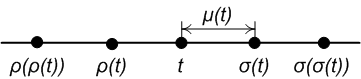
\includegraphics[width=0.4\paperwidth]{operators}
}

\frame{
	La integración se define de modo que $\int_{t}^{s}f^{\Delta}\left(\tau\right)\Delta\tau=f\left(t\right)-f\left(s\right)$.

	Si $\mathds{T}$ consiste únicamente de puntos aislados, entonces \[ f^{\Delta}\left(t\right)=\frac{f\left(\sigma\left(t\right)\right)-f\left(t\right)}{\mu\left(t\right)} \]

	y

\[
\int_{a}^{b}f\left(t\right)\Delta t=
\begin{cases}
	\sum_{t\in\left[a,b\right)\cap\mathds{T}}\mu\left(t\right)f\left(t\right),&\text{si }a<b.\\
	0, & \text{si } a = b.\\
	-\sum_{t\in\left[b,a\right)\cap\mathds{T}}\mu\left(t\right)f\left(t\right), & \text{si }a>b.
	\end{cases}
\]
}
%%%%%%%%%%%%%%%%%%%%%%%%%%%%%%%%%%%%%%%%%%%%%%%%%%%%%%%%%%%%%%%%%
\renewcommand{\refname}{Referencias bibliográficas}
\nocite{*}
\bibliographystyle{spmpsci}
{\footnotesize 
	\bibliography{bib}}
%[title={Referencias bibliográficas},heading=bibintoc]}
%\biblstarthook{In view of the parallel print and (chapter-wise) online publication of your book at \url{www.springerlink.com} it has been decided that -- as a genreral rule --  references should be sorted chapter-wise and placed at the end of the individual chapters. However, upon agreement with your contact at Springer you may list your references in a single seperate chapter at the end of your book. Deactivate the class option \texttt{sectrefs} and the \texttt{thebibliography} environment will be put out as a chapter of its own.\\\indent
%References may be \textit{cited} in the text either by number (preferred) or by author/year.\footnote{Make sure that all references from the list are cited in the text. Those not cited should be moved to a separate \textit{Further Reading} section or chapter.} If the citatiion in the text is numbered, the reference list should be arranged in ascending order. If the citation in the text is author/year, the reference list should be \textit{sorted} alphabetically and if there are several works by the same author, the following order should be used:
\begin{frame}
\frametitle{Agradecimientos}

\begin{center}\Large
	¡Muchas gracias!
\end{center}

Colaboradores:

\begin{enumerate}
	\item Creación del módulo \texttt{timescalecalculus}: Dr. Tom Cuchta y Matthias Baur.
	\item Tipografía en \LaTeX{}: Todo el grupo.
	\item Explicación del contenido matemático: Todo el grupo.
	\item Esquema de la exposición: Todo el grupo.
\end{enumerate}

\

{
\color{DarkBlue}
Presentación disponible en:
}
\begin{center}
\href{https://github.com/carlosal1015/Real-Analysis-Project}{
\includegraphics[width=2.5cm]{Octocat.png}}
\end{center}
\hfill
\begin{flushright}
Dudas, sugerencias o preguntas a

\href{mailto:caznaranl@uni.pe}{caznaranl\MVAt uni.pe}
\end{flushright}
\end{frame}

%\justfor{student}{
%	
%}
%\includeslide{}
%\appendix
%\frame[noframenumbering,plain]{text}
\end{document}
https://www.i-ciencias.com/pregunta/35252/termino-comun-para-las-ecuaciones-diferenciales-y-de-relaciones-de-recurrencia

@book{book:{2135209},
	title =     {Intelligent computations : abstract fractional calculus, inequalities, approximations},
	author =    {Anastassiou, George A},
	publisher = {Springer},
	isbn =      { 978-3-319-66936-6,3319669362,978-3-319-66935-9 },
	year =      {2018},
	series =    {Studies in computational intelligence 734},
	edition =   {},
	volume =    {},
	url =       {http://gen.lib.rus.ec/book/index.php?md5=edcebea5cf073b0368a47fba1cb9b635}}

Dada la ecuación en diferencias lineal de coeficientes constantes y de orden $k$: $a_{0}f(n + k)+a_{1}f(n+k¡1)+\cdots+a_{k}f(n)=g(n)$, el problema de hallar una función $f$ definida en $\mathds{Z}$; que verifique la ecuación, y tal que en los $k$ enteros consecutivos $n_{0},n_{0}+1,\ldots,n_{0}+k-1$ tome los valores dados $c_{0},c_{1},\ldots,c_{k-1}$; tiene solución única.
%\sectionmark{Ejercicios}
\section*{Ejercicios}
\begin{prob}{Sucesión contractiva}
	Una sucesión $\left\{x_{n}\right\}$ se dice que \textbf{contractiva} si $\exists$ alguna constante $c$, $0<c<1\ni\forall\,n\in\mathds{N}$, $|x_{n+2}-x_{n+1}|\leq c|x_{n+1}-x_{n}|$. Pruebe que una sucesión contractiva debe ser una sucesión de Cauchy, y por lo tanto converge.
\end{prob}

\begin{prob}{Media aritmética recursiva}
Sea $a\neq b$ números reales arbitrarios, y defina la sucesión $\left\{x_{n}\right\}$ por \[ x_{1}=a,x_{2}=b,\text{ y }\forall\,n\in\mathds{N},x_{n+2}=\frac{x_{n+1}+x_{n}}{2}. \] Esto es, cada nuevo término está iniciando con el tercero que es el promedio de los dos términos previos.
	\begin{enumerate}
		\item Pruebe que $\left\{x_{n}\right\}$ converge probando que este es una sucesión constructiva.
		\item Pruebe que $\forall\,n\in\mathds{N}$, $x_{n+1}+\frac{1}{2}x_{n}=b+\frac{1}{2}a$.\label{9b}
		\item Use~\ref{9b} y el álgebra de límites para encontrar que  $\lim\limits_{n\to\infty}x_{n}$. ?`Está sorprendido por la respuesta? Note que si usted intercambia $a$ y $b$ la respuesta podría ser diferente.
	\end{enumerate}
\end{prob}

\begin{prob}{Media aritmética ponderada recursiva}
	Sean $a\neq b$ dos números reales arbitrarios, sea $0<t<1$, y defina la sucesión $\left\{x_{n}\right\}$ por \[ x_{1}=a,x_{2}=b,\text{ z }\forall\,n\in\mathds{N},x_{n+2}=tx_{n}+\left(1-t\right)x_{n+1}. \] Esto es, cada nuevo término que inicia con el tercero que es el promedio ponderado de los términos previos. Geométricamente, $x_{n+2}$ es un punto en el intervalo entre $x_{n}$ y $x_{n+1}$ que corta el intervalo en dos segmentos cuyas longitudes están en la proporción $t$ a $1-t$. Pruebe que $\left\{x_{n}\right\}$ es contractiva, y encuentre su límite.
\end{prob}

\begin{prob}{Aplicación contractiva}
	Sean $a<b$ e $I=\left[a,b\right]$. Una función $f\colon I\rightarrow I$ se dice que es una \textbf{contracción} si $\exists c\ni0<c<1$ y $\forall\,x,y\in I$, $|f\left(x\right)-f\left(y\right)|\leq c|x-y|$. Pruebe que una aplicación contractiva debe tener por lo menos un ``punto fijo'', $x\in I\ni f\left(x\right)=x$. También pruebe que $f$ no puede tener más de un punto fijo en $I$.
\end{prob}

\begin{prob}{Números de Fibonacci}
	La sucesión de Fibonacci consiste de los números de Fibonacci, $1,1,2,3,5,8,13,21,\ldots$, y está definido recursivamente por $f_{1}=1$, $f_{2}=1$, y $\forall\,n\geq2$, $f_{n+2}=f_{n+1}+f_{n}$. Cada nuevo término después del segundo es la suma de los dos términos previos. Muchos resultados interesantes han sido probados acerca de los números de Fibonacci--lo suficiente para llenar un libro entero. Deberemos concentrarnos aquí con la sucesión de proporciones de los sucesivos números de Fibonacci. Empezamos definiendo la sucesión por $r_{n}=\tfrac{f_{n+1}}{f_{n}}$.
		\begin{enumerate}
			\item Desarrolle una tabla que muestre los primeros diez términos de $\left\{r_{n}\right\}$. En la basa de esta tabla, conjeture las respuestas a las siguientes preguntas. ?`$\left\{r_{n}\right\}$ es convergente? ?`Es monótona? ?`Eventualmente monótona? ?`Puede encontrar una subsucesión estrictamente creciente? ?`Una subsucesión estrictamente decreciente? (No se requieren demostraciones).
			\item Pruebe que $\forall\,n\in\mathds{N}$, $r_{n+1}=1+\tfrac{1}{r_{n}}$.
			\item Pruebe que $\forall\,n\geq2$, $\tfrac{3}{2}<r_{n}<2$.
			\item Pruebe que $\left\{r_{n}\right\}$ es ``contractiva'', y por lo tanto es una sucesión de Cauchy.
			\item Encuentre $\lim\limits_{n\to\infty}r_{n}$. [Tome nota de este límite; este reaparecerá.]
			\item La ecuación cuadrática $x^{2}-x-1=0$ tiene dos soluciones, $\alpha=\frac{1+\sqrt{5}}{2}$ y $\beta=\frac{1-\sqrt{5}}{2}$. Muestre que $\alpha+\beta=1$, $\alpha^{2}=a+1$, y $\beta^{2}=\beta+1$, y desde estos hechos muestre que $\forall\,n\in\mathbb{N}$, $\alpha^{n+2}=\alpha^{n+1}+\alpha^{n}$ y $\beta^{n+2}=\beta^{n+1}+\beta^{n}$.\label{9f}
			\item $\forall\,n\in\mathds{N}$, defina $u_{n}=\frac{\alpha^{n}-\beta^{n}}{\alpha-\beta}$, donde $\alpha$ y $\beta$ están definidos en~\ref{9f}. Pruebe que $u_{1}=1$, $u_{2}=1$, y $\forall\,n\geq2$, $u_{n+2}=u_{n+1}+u_{n}$. Por lo tanto, $\left\{u_{n}\right\}$ debe ser la sucesión de Fibonacci. Tenemos encontrado una fórmula para los números de Fibonacci: $f_{n}=u_{n}$.
			\item \textbf{Significado geométrico} de $\alpha$. Considere un rectángulo cuyo ancho $\alpha$ y largo $a+b$ son así proporcionados que cuando un cuadrado de lado $a$ es removido, como se muestra aquí, el rectángulo restante tiene ancho y longitud en la misma proporción. Esto es, $\tfrac{a+b}{a}=\tfrac{a}{b}$.
	
			Los matemáticos de la Grecia clásica llamaron esta proporción $R=\frac{a}{b}$ la ``\textbf{Proporción áurea}'' y cualquier rectángulo con lados en la proporción un ``\textbf{rectángulo áureo}''. Ellos consideraron esto como la más estéticamente agradable de todos los rectángulos, y se usó esto frecuentemente en su arte y arquitectura. Pruebe algebraicamente que $R=\alpha$, definida en~\ref{9f} arriba.
			\item Pruebe que $\forall\,n\geq2$, $\forall\,n\geq2$, $f_{n+1}f_{n-1}-{\left(f_{n}\right)}^{2}={\left(-1\right)}^{n}$.
			\item Pruebe que $\forall\,n\in\mathds{N}$, $r_{n+1}-r_{n}=\frac{{\left(-1\right)}^{n+1}}{f_{n}f_{n+1}}$.\label{9j}
			\item Use~\ref{9j} para probar que $\left\{r_{2n}\right\}$ es estrictamente decreciente y $\left\{r_{2n+1}\right\}$ es estrictamente creciente.
	\end{enumerate}
\end{prob}

\begin{prob}{}
	Sea $a\geq1$. Defina la sucesión $\left\{x_{n}\right\}$ por $x_{1}=a$, y $x_{n+1}=a+\frac{1}{x_{m}}$. Pruebe que $\forall\,n\geq2$, $a+\frac{1}{2a}\leq x_{n}\leq 2a$, y use este resultado para probar que $x_{n}$ es contractiva. Encuentre $\lim\limits_{n\to\infty}x_{n}$.
\end{prob}

\begin{prob}{}
	Sea $a>1$. Defina la sucesión $\left\{x_{n}\right\}$ por $x_{1}=a$ y $x_{n}=\frac{1}{a+x_{n}}$. Pruebe que $\forall\,n\in\mathds{N}$, $\frac{1}{2a}\leq x_{n}\leq a$, y use este resultado para probar que $\left\{x_{n}\right\}$ es contractiva. Encuentre el $\lim\limits_{n\to\infty}x_{n}$. Compare este límite con el ejercicio anterior.
\end{prob}
%%\motto{Use the template \emph{chapter.tex} to style the various elements of your chapter content.}
%\chapter{}
%\label{intro} % Always give a unique label
% use \chaptermark{}
% to alter or adjust the chapter heading in the running head
%
%\abstract*{}
%
%\abstract{El cálculo de variaciones se desarrolló a partir del problema de la curva braquistócrona, planteado inicialmente por \textbf{Johann Bernoulli} (1696). Inmediatamente este problema captó la atención de Jakob Bernoulli y el marqués de l'Hôpital, aunque fue \textbf{Leonhard Euler} el primero que elaboró una teoría del cálculo variacional. Las contribuciones de Euler se iniciaron en 1733 con su Elementa Calculi Variationum (``Elementos del cálculo de variaciones'') que da nombre a la disciplina. \newline\indent
%\textbf{Lagrange} contribuyó extensamente a la teoría y Legendre (1786) asentó un método, no enteramente satisfactorio para distinguir entre máximos y mínimos. \textbf{Isaac Newton} y \textbf{Gottfried Leibniz} también prestaron atención a este asunto.}
%
%\section{Otras publicaciones}
%\label{sec:1}
%Otros trabajos destacados fueron los de Vincenzo Brunacci (1810), Carl Friedrich Gauss (1829), Siméon Poisson (1831), Mijaíl Ostrogradski (1834) y Carl Jacobi (1837). Un trabajo general particularmente importante es el de Sarrus (1842) que fue resumido por Cauchy (1844). Otros trabajos destacados posteriores son los de Strauch (1849), Jellett (1850), Otto Hesse (1857), Alfred Clebsch (1858) y Carll (1885), aunque quizá el más importante de los trabajos durante el siglo XIX es el de \textbf{Weierstrass}. Este importante trabajo fue una referencia estándar y es el primero que trata el cálculo de variaciones sobre una base firme y rigurosa. Los problema 20 y 23 de Hilbert planteados en 1900 estimularon algunos desarrollos posteriores. Durante el siglo XX, David Hilbert, Emmy Noether, Leonida Tonelli, Henri Lebesgue y Jacques Hadamard, entre otros, hicieron contribuciones notables.\par
%\textbf{Marston Morse} aplicó el cálculo de variaciones a lo que actualmente se conoce como teoría de Morse. Lev Semenovich Pontryagin, Ralph Rockafellar y Clarke desarrollaron nuevas herramientas matemáticas dentro de la teoría del control óptimo, generalizando el cálculo de variaciones.
%
%\section{Fermat, Bernoulli, Newton y Leibniz}
%\label{sec:2}
%% Always give a unique label
%% and use \ref{<label>} for cross-references
%% and \cite{<label>} for bibliographic references
%% use \sectionmark{}
%%% to alter or adjust the section heading in the running head
%%
%%% For figures use
%%%
%\begin{figure}[!ht]
%	\sidecaption[t]
%	% Use the relevant command for your figure-insertion program
%	% to insert the figure file.
%	% For example, with the option graphics use
%	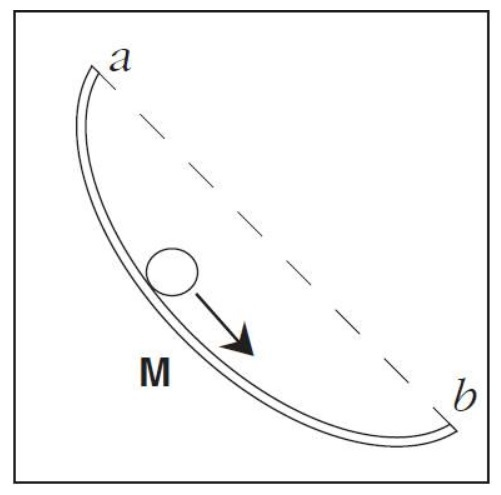
\includegraphics[width=0.343\textwidth]{bola.jpg}
%	%
%	% If not, use
%	%\picplace{5cm}{2cm} % Give the correct figure height and width in cm
%	%
%	\caption{Dados dos puntos $A$ y $B$, con $A$ a una elevación mayor que $B$, existe solo una curva cicloide con la concavidad hacia arriba que pasa por $A$ con pendiente infinita (dirección vertical y sentido de arriba hacia abajo), también pasa por $B$ y no posee puntos máximos entre $A$ y $B$.}
%	\label{fig:1}       % Give a unique label
%\end{figure}
%
%\eject
%
%%\begin{eqnarray}
%%\left|\nabla U_{\alpha}^{\mu}(y)\right| &\le&\frac1{d-\alpha}\int
%%\left|\nabla\frac1{|\xi-y|^{d-\alpha}}\right|\,d\mu(\xi) =
%%\int \frac1{|\xi-y|^{d-\alpha+1}} \,d\mu(\xi)\qquad  \\
%%&=&(d-\alpha+1) \int\limits_{d(y)}^\infty
%%\frac{\mu(B(y,r))}{r^{d-\alpha+2}}\,dr \le (d-\alpha+1)
%%\int\limits_{d(y)}^\infty \frac{r^{d-\alpha}}{r^{d-\alpha+2}}\,dr
%%\label{eq:01}
%%\end{eqnarray}
%
%\enlargethispage{24pt}
%
%\begin{quotation}
%Please do not use quotation marks when quoting texts! Simply use the \verb|quotation| environment -- it will automatically be rendered in the preferred layout.
%\end{quotation}
%\subsection{Algunas observaciones, demostraciones y aplicaciones de Euler, Lagrange y Jacobi en el Cálculo variacional}
%Instead of simply listing headings of different levels we recommend to let every heading be followed by at least a short passage of text. Furtheron please use the \LaTeX\ automatism for all your cross-references and citations as has already been described in Sect.~\ref{subsec:2}, see also Fig.~\ref{fig:1}\footnote{If you copy text passages, figures, or tables from other works, you must obtain \textit{permission} from the copyright holder (usually the original publisher). Please enclose the signed permission with the manucript. The sources\index{permission to print} must be acknowledged either in the captions, as footnotes or in a separate section of the book.}
%\paragraph{Paragraph Heading} %
%Instead of simply listing headings of different levels we recommend to let every heading be followed by at least a short passage of text. Furtheron please use the \LaTeX\ automatism for all your cross-references and citations as has already been described in Sect.~\ref{sec:2}.
%
%Please note that the first line of text that follows a heading is not indented, whereas the first lines of all subsequent paragraphs are.
%
%For typesetting numbered lists we recommend to use the \verb|enumerate| environment -- it will automatically render Springer's preferred layout.
%\begin{figure}[h]
%	\centering
%	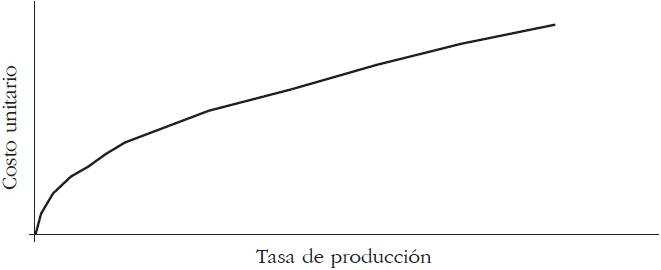
\includegraphics[width=0.6\textwidth]{grafica.jpg}
%	\caption{Costo de producción proporcional a la raíz cuadrada de la tasa de producción.}
%\end{figure}
%\begin{figure}[t]
%\sidecaption[t]
%% Use the relevant command for your figure-insertion program
%% to insert the figure file.
%% For example, with the option graphics use
%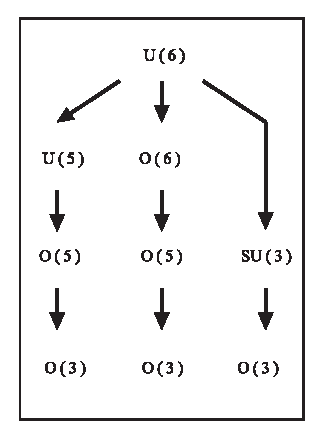
\includegraphics[scale=.65]{figure}
%%
%% If not, use
%%\picplace{5cm}{2cm} % Give the correct figure height and width in cm
%%
%\caption{Please write your figure caption here}
%\label{fig:2}       % Give a unique label
%\end{figure}
%
%\runinhead{Run-in Heading Boldface Version} Use the \LaTeX\ automatism for all your cross-references and citations as has already been described in Sect.~\ref{sec:2}.
%
%\subruninhead{Run-in Heading Boldface and Italic Version} Use the \LaTeX\ automatism for all your cross-refer\-ences and citations as has already been described in Sect.~\ref{sec:2}\index{paragraph}.
%
%\subsubruninhead{Run-in Heading Displayed Version} Use the \LaTeX\ automatism for all your cross-refer\-ences and citations as has already been described in Sect.~\ref{sec:2}\index{paragraph}.
%% Use the \index{} command to code your index words
%%
%% For tables use
%%
%\begin{table}[!t]
%\caption{Please write your table caption here}
%\label{tab:1}       % Give a unique label
%%
%% For LaTeX tables use
%%
%\begin{tabular}{p{2cm}p{2.4cm}p{2cm}p{4.9cm}}
%\hline\noalign{\smallskip}
%Classes & Subclass & Length & Action Mechanism  \\
%\noalign{\smallskip}\svhline\noalign{\smallskip}
%Translation & mRNA$^a$  & 22 (19--25) & Translation repression, mRNA cleavage\\
%Translation & mRNA cleavage & 21 & mRNA cleavage\\
%Translation & mRNA  & 21--22 & mRNA cleavage\\
%Translation & mRNA  & 24--26 & Histone and DNA Modification\\
%\noalign{\smallskip}\hline\noalign{\smallskip}
%\end{tabular}
%$^a$ Table foot note (with superscript)
%\end{table}
%%
%\section{Section Heading}
%\label{sec:3}
%% Always give a unique label
%% and use \ref{<label>} for cross-references
%% and \cite{<label>} for bibliographic references
%% use \sectionmark{}
%% to alter or adjust the section heading in the running head
%Instead of simply listing headings of different levels we recommend to let every heading be followed by at least a short passage of text. Furtheron please use the \LaTeX\ automatism for all your cross-references and citations as has already been described in Sect.~\ref{sec:2}.
%
%Please note that the first line of text that follows a heading is not indented, whereas the first lines of all subsequent paragraphs are.
%
%If you want to list definitions or the like we recommend to use the Springer-enhanced \verb|description| environment -- it will automatically render Springer's preferred layout.
%
%\begin{description}[Type 1]
%\item[Type 1]{That addresses central themes pertainng to migration, health, and disease. In Sect.~\ref{sec:1}, Wilson discusses the role of human migration in infectious disease distributions and patterns.}
%\item[Type 2]{That addresses central themes pertainng to migration, health, and disease. In Sect.~\ref{subsec:2}, Wilson discusses the role of human migration in infectious disease distributions and patterns.}
%\end{description}
%
%\subsection{Subsection Heading} %
%In order to avoid simply listing headings of different levels we recommend to let every heading be followed by at least a short passage of text. Use the \LaTeX\ automatism for all your cross-references and citations citations as has already been described in Sect.~\ref{sec:2}.
%
%Please note that the first line of text that follows a heading is not indented, whereas the first lines of all subsequent paragraphs are.
%
%\begin{svgraybox}
%If you want to emphasize complete paragraphs of texts we recommend to use the newly defined Springer class option \verb|graybox| and the newly defined environment \verb|svgraybox|. This will produce a 15 percent screened box 'behind' your text.
%
%If you want to emphasize complete paragraphs of texts we recommend to use the newly defined Springer class option and environment \verb|svgraybox|. This will produce a 15 percent screened box 'behind' your text.
%\end{svgraybox}
%
%
%\subsubsection{Subsubsection Heading}
%Instead of simply listing headings of different levels we recommend to let every heading be followed by at least a short passage of text. Furtheron please use the \LaTeX\ automatism for all your cross-references and citations as has already been described in Sect.~\ref{sec:2}.
%
%Please note that the first line of text that follows a heading is not indented, whereas the first lines of all subsequent paragraphs are.
%
%\begin{theorem}
%Theorem text goes here.
%\end{theorem}
%%
%% or
%%
%\begin{definition}
%Definition text goes here.
%\end{definition}
%
%\begin{proof}
%%\smartqed
%Proof text goes here.
%%\qed
%\end{proof}
%
%\paragraph{Paragraph Heading} %
%Instead of simply listing headings of different levels we recommend to let every heading be followed by at least a short passage of text. Furtheron please use the \LaTeX\ automatism for all your cross-references and citations as has already been described in Sect.~\ref{sec:2}.
%
%Note that the first line of text that follows a heading is not indented, whereas the first lines of all subsequent paragraphs are.
%%
%% For built-in environments use
%%
%\begin{theorem}
%Theorem text goes here.
%\end{theorem}
%%
%\begin{definition}
%Definition text goes here.
%\end{definition}
%%
%\begin{proof}
%%\smartqed
%Proof text goes here.
%%\qed
%\end{proof}
%%
%%
%\begin{trailer}{Cabeza de remolque}
%If you want to emphasize complete paragraphs of texts in an \verb|Trailer Head| we recommend to
%use  \begin{verbatim}\begin{trailer}{Trailer Head}
%...
%\end{trailer}\end{verbatim}
%\end{trailer}
%%
%\begin{question}{Preguntas}
%If you want to emphasize complete paragraphs of texts in an \verb|Questions| we recommend to
%use  \begin{verbatim}\begin{question}{Questions}
%...
%\end{question}\end{verbatim}
%\end{question}
%%
%%
%\begin{important}{Importante}
%If you want to emphasize complete paragraphs of texts in an \verb|Important| we recommend to
%use  \begin{verbatim}\begin{important}{Important}
%...
%\end{important}\end{verbatim}
%\end{important}
%%
%\clearpage
%\begin{warning}{Atención}
%If you want to emphasize complete paragraphs of texts in an \verb|Attention| we recommend to
%use  \begin{verbatim}\begin{warning}{Attention}
%...
%\end{warning}\end{verbatim}
%\end{warning}
%
%\begin{programcode}{Código de programa}
%If you want to emphasize complete paragraphs of texts in an \verb|Program Code| we recommend to
%use
%
%\verb|\begin{programcode}{Program Code}|
%
%\verb|\begin{verbatim}...\end{verbatim}|
%
%\verb|\end{programcode}|
%
%\end{programcode}
%%
%\begin{tips}{Consejos}
%If you want to emphasize complete paragraphs of texts in an \verb|Tips| we recommend to
%use  \begin{verbatim}\begin{tips}{Tips}
%...
%\end{tips}\end{verbatim}
%\end{tips}
%%
%%
%\begin{overview}{Visión general}
%If you want to emphasize complete paragraphs of texts in an \verb|Overview| we recommend to
%use  \begin{verbatim}\begin{overview}{Overview}
%...
%\end{overview}\end{verbatim}
%\end{overview}
%\clearpage
%\begin{backgroundinformation}{Background Information}
%If you want to emphasize complete paragraphs of texts in an \verb|Background|
%\verb|Information| we recommend to
%use
%
%\verb|\begin{backgroundinformation}{Background Information}|
%
%\verb|...|
%
%\verb|\end{backgroundinformation}|
%\end{backgroundinformation}
%\begin{legaltext}{Legal Text}
%If you want to emphasize complete paragraphs of texts in an \verb|Legal Text| we recommend to
%use  \begin{verbatim}\begin{legaltext}{Legal Text}
%...
%\end{legaltext}\end{verbatim}
%\end{legaltext}
%%
%\begin{acknowledgement}
%If you want to include acknowledgments of assistance and the like at the end of an individual chapter please use the \verb|acknowledgement| environment -- it will automatically render Springer's preferred layout.
%\end{acknowledgement}
%%
%\section*{Apéndice}
%\addcontentsline{toc}{section}{Apéndice}
%%
%When placed at the end of a chapter or contribution (as opposed to at the end of the book), the numbering of tables, figures, and equations in the appendix section continues on from that in the main text. Hence please \textit{do not} use the \verb|appendix| command when writing an appendix at the end of your chapter or contribution. If there is only one the appendix is designated ``Appendix'', or ``Appendix 1'', or ``Appendix 2'', etc. if there is more than one.
%
%\begin{equation}
%a \times b = c
%\end{equation}
%% Problems or Exercises should be sorted chapterwise
%\section*{Problemas}
%\addcontentsline{toc}{section}{Problems}
%%
%% Use the following environment.
%% Don't forget to label each problem;
%% the label is needed for the solutions' environment
%\begin{prob}
%\label{prob1}
%A given problem or Excercise is described here. The
%problem is described here. The problem is described here.
%\end{prob}
%
%\begin{prob}
%\label{prob2}
%\textbf{Problem Heading}\\
%(a) The first part of the problem is described here.\\
%(b) The second part of the problem is described here.
%\end{prob}
\renewcommand{\refname}{Referencias bibliográficas}
\nocite{*}
\bibliographystyle{spmpsci}
{\footnotesize 
	\bibliography{bib}}
%[title={Referencias bibliográficas},heading=bibintoc]}
%\biblstarthook{In view of the parallel print and (chapter-wise) online publication of your book at \url{www.springerlink.com} it has been decided that -- as a genreral rule --  references should be sorted chapter-wise and placed at the end of the individual chapters. However, upon agreement with your contact at Springer you may list your references in a single seperate chapter at the end of your book. Deactivate the class option \texttt{sectrefs} and the \texttt{thebibliography} environment will be put out as a chapter of its own.\\\indent
%References may be \textit{cited} in the text either by number (preferred) or by author/year.\footnote{Make sure that all references from the list are cited in the text. Those not cited should be moved to a separate \textit{Further Reading} section or chapter.} If the citatiion in the text is numbered, the reference list should be arranged in ascending order. If the citation in the text is author/year, the reference list should be \textit{sorted} alphabetically and if there are several works by the same author, the following order should be used:
%\appendix
\motto{All's well that ends well}
%\chapter{Chapter Heading}
%\label{introA} % Always give a unique label
% use \chaptermark{}
% to alter or adjust the chapter heading in the running head

\section{Section Heading}
\label{sec:A1}
% Always give a unique label
% and use \ref{<label>} for cross-references
% and \cite{<label>} for bibliographic references
% use \sectionmark{}
% to alter or adjust the section heading in the running head
Instead of simply listing headings of different levels we recommend to let every heading be followed by at least a short passage of text. Furtheron please use the \LaTeX\ automatism for all your cross-references and citations.

\subsection{Subsection Heading}
\label{sec:A2}
Instead of simply listing headings of different levels we recommend to let every heading be followed by at least a short passage of text. Furtheron please use the \LaTeX\ automatism for all your cross-references and citations as has already been described in Sect.~\ref{sec:A1}.

For multiline equations we recommend to use the \verb|eqnarray| environment.
\begin{eqnarray}
\vec{a}\times\vec{b}=\vec{c} \nonumber\\
\vec{a}\times\vec{b}=\vec{c}
\label{eq:A01}
\end{eqnarray}

\subsubsection{Subsubsection Heading}
Instead of simply listing headings of different levels we recommend to let every heading be followed by at least a short passage of text. Furtheron please use the \LaTeX\ automatism for all your cross-references and citations as has already been described in Sect.~\ref{sec:A2}.

Please note that the first line of text that follows a heading is not indented, whereas the first lines of all subsequent paragraphs are.

% For figures use
%
\begin{figure}[t]
\sidecaption[t]
%\centering
% Use the relevant command for your figure-insertion program
% to insert the figure file.
% For example, with the option graphics use
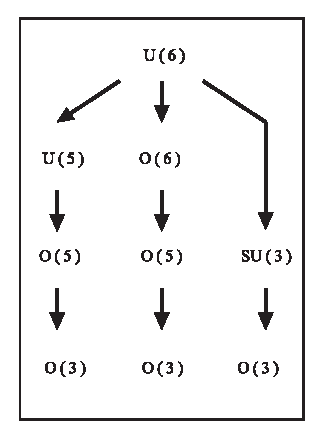
\includegraphics[scale=.65]{figure}
%
% If not, use
%\picplace{5cm}{2cm} % Give the correct figure height and width in cm
%
\caption{Please write your figure caption here}
\label{fig:A1}       % Give a unique label
\end{figure}

% For tables use
%
\begin{table}
\caption{Please write your table caption here}
\label{tab:A1}       % Give a unique label
%
% For LaTeX tables use
%
\begin{tabular}{p{2cm}p{2.4cm}p{2cm}p{4.9cm}}
\hline\noalign{\smallskip}
Classes & Subclass & Length & Action Mechanism  \\
\noalign{\smallskip}\hline\noalign{\smallskip}
Translation & mRNA$^a$  & 22 (19--25) & Translation repression, mRNA cleavage\\
Translation & mRNA cleavage & 21 & mRNA cleavage\\
Translation & mRNA  & 21--22 & mRNA cleavage\\
Translation & mRNA  & 24--26 & Histone and DNA Modification\\
\noalign{\smallskip}\hline\noalign{\smallskip}
\end{tabular}
$^a$ Table foot note (with superscript)
\end{table}
\renewcommand{\refname}{Referencias bibliográficas}
\nocite{*}
\bibliographystyle{spmpsci}
{\footnotesize 
	\bibliography{bib}}
%[title={Referencias bibliográficas},heading=bibintoc]}
%\biblstarthook{In view of the parallel print and (chapter-wise) online publication of your book at \url{www.springerlink.com} it has been decided that -- as a genreral rule --  references should be sorted chapter-wise and placed at the end of the individual chapters. However, upon agreement with your contact at Springer you may list your references in a single seperate chapter at the end of your book. Deactivate the class option \texttt{sectrefs} and the \texttt{thebibliography} environment will be put out as a chapter of its own.\\\indent
%References may be \textit{cited} in the text either by number (preferred) or by author/year.\footnote{Make sure that all references from the list are cited in the text. Those not cited should be moved to a separate \textit{Further Reading} section or chapter.} If the citatiion in the text is numbered, the reference list should be arranged in ascending order. If the citation in the text is author/year, the reference list should be \textit{sorted} alphabetically and if there are several works by the same author, the following order should be used:

\backmatter%%%%%%%%%%%%%%%%%%%%%%%%%%%%%%%%%%%%%%%%%%%%%%%%%%%%%%%
%\Extrachap{Glosario}

\runinhead{término del glosario}
%
\Extrachap{Soluciones}

\section*{Problemas del Capítulo~\ref{intro}}

\begin{sol}{prob1}
The solution\index{problems}\index{solutions} is revealed here.
\end{sol}


\begin{sol}{prob2}
\textbf{Problem Heading}\\
(a) The solution of first part is revealed here.\\
(b) The solution of second part is revealed here.
\end{sol}



\printindex

%%%%%%%%%%%%%%%%%%%%%%%%%%%%%%%%%%%%%%%%%%%%%%%%%%%%%%%%%%%%%%%%%%%%%%
\end{document}